\documentclass[preprint,3p,10pt]{elsarticle}




%------------------------------------------------------------------------------
% FIGURES: CHOOSE ONE OPTION
%
% plots:       build standalone pdfs for figures, then use them
% plots-ext:   use existing pdfs for figures
% plots-none:  skip figures
%
\input{tex/plots}
%------------------------------------------------------------------------------
% space before \paragraph (default 4.05ex)
% \makeatletter
% \renewcommand\paragraph{\@startsection{paragraph}{4}{\z@}{1ex}{-1em}{\normalfont\normalsize\bfseries}}
% \makeatother
%------------------------------------------------------------------------------
% \usepackage[numbers,sort&compress]{natbib}
\usepackage{natbib}
\usepackage{times}
\usepackage{epsfig}
\usepackage{graphicx}
\usepackage{amsmath}
\usepackage{amssymb}
\usepackage{xspace}
\usepackage{color}
% \usepackage{setspace} 

\usepackage{enumitem}
\usepackage{multirow}
\usepackage{array,booktabs}
\usepackage{bbm}
\usepackage{colortbl}

\usepackage[pagebackref=true,breaklinks=true,colorlinks,bookmarks=false]{hyperref}

% Support for easy cross-referencing
\usepackage[capitalize]{cleveref}
\crefname{section}{Sec.}{Secs.}
\Crefname{section}{Section}{Sections}
\Crefname{table}{Table}{Tables}
\crefname{table}{Tab.}{Tabs.}

\journal{Pattern Recognition}
% \doublespacing
\linespread{2}
\begin{document}


\input{tex/abbrev}
% \newcommand{\func}[1]{\mathsf{#1}}
% \def \ff {\func{f}}
% \def \fa {\func{a}}
% \def \fb {\func{b}}
% \def \fc {\func{c}}
% \def \fs {\func{s}}
% \def \fP {\func{P}}
% \def \fT {\func{T}}
% \def \fR {\func{R}}
% \def \fL {\func{L}}



\newcommand{\relu}{\operatorname{relu}}
\newcommand{\gap}{\operatorname{GAP}}
\newcommand{\up}{\operatorname{up}}

\newcommand{\cam}{\textrm{CAM}}
\newcommand{\gcam}{\textrm{Grad-CAM}}
\newcommand{\scam}{\textrm{Score-CAM}}

\newcommand{\Fdef}{Mask\xspace}
\newcommand{\Fref}{Diff\xspace}
\newcommand{\MIOFref}{IODiff\xspace}
\newcommand{\MIODref}{IOMask\xspace}


\newcommand{\AG}{\operatorname{AG}}
\newcommand{\AGf}{Average Gain\xspace}
\newcommand{\Agf}{Average gain\xspace}
\newcommand{\agf}{average gain\xspace}

\newcommand{\AC}{\operatorname{AC}}
\newcommand{\ACf}{Average Contract\xspace}

\newcommand{\AD}{\operatorname{AD}}
\newcommand{\I}{\operatorname{I}}
\newcommand{\D}{\operatorname{D}}
\newcommand{\AI}{\operatorname{AI}}
\newcommand{\OM}{\operatorname{OM}}
\newcommand{\LE}{\operatorname{LE}}
\newcommand{\Fo}{\operatorname{F1}}
\newcommand{\prc}{\operatorname{precision}}
\newcommand{\rec}{\operatorname{recall}}
\newcommand{\BA}{\operatorname{BoxAcc}}
\newcommand{\spg}{\operatorname{SP}}
\newcommand{\epg}{\operatorname{EP}}
\newcommand{\SM}{\operatorname{SM}}
\newcommand{\iou}{\operatorname{IoU}}



\newcommand{\ronan}[1]{#1}
\newcommand{\iavr}[1]{#1}
\newcommand{\stephane}[1]{#1}
\newcommand{\redred}[1]{#1}
\newcommand{\hw}[1]{{\color{olive}{#1}}}
% \newcommand{\modify}[1]{{\color{blue}{#1}}}
\newcommand{\modify}[1]{{{#1}}}


\begin{frontmatter}
\title{Opti-CAM: Optimizing saliency maps for interpretability}


\author[1]{Hanwei Zhang}
\ead{hanwei.zhang@lis-lab.fr}
% \cormark[1]
\author[1]{Felipe Torres}
\ead{felipe.torres@lis-lab.fr}
\author[1]{Ronan Sicre}
\ead{ronan.sicre@lis-lab.fr}
\author[2]{Yannis Avrithis}
\ead{yannis@avrithis.net}
\author[1]{Stephane Ayache}
\ead{stephane.ayache@univ-amu.fr}


% Address/affiliation
\affiliation[1]{organization={Centrale Marseille, Aix Marseille Univ, CNRS, LIS},
            % addressline={52 Av. Escadrille Normandie Niemen}, 
            city={Marseille},
%          citysep={}, % Uncomment if no comma needed between city and postcode
            postcode={13397}, 
            % state={},
            country={France}}

\affiliation[2]{organization={Institute of Advanced Research on Artificial Intelligence (IARAI)},
            % addressline={Landstraßer Hauptstraße 5 Eingang, u. Viaduktgasse 16, 2. Stock}, 
            city={Vienna},
%          citysep={}, % Uncomment if no comma needed between city and postcode
            postcode={1030}, 
            % state={},
            country={Austria}}



\begin{abstract}
Methods based on \emph{class activation maps} (CAM) provide a simple mechanism to interpret predictions of convolutional neural networks by using linear combinations of feature maps as saliency maps. By contrast, masking-based methods optimize a saliency map directly in the image space or learn it by training another network on additional data.

In this work we introduce Opti-CAM, combining ideas from CAM-based and masking-based approaches. Our saliency map is a linear combination of feature maps, where weights are optimized per image such that the logit of the masked image for a given class is maximized. We also fix a fundamental flaw in two of the most common evaluation metrics of attribution methods. On several datasets, Opti-CAM largely outperforms other CAM-based approaches according to the most relevant classification metrics. We provide empirical evidence supporting that localization and classifier interpretability are not necessarily aligned.
\end{abstract}

% \begin{graphicalabstract}
% \end{graphicalabstract}

\begin{highlights}
\item We introduce Opti-CAM, a simple model for saliency map generation that combines ideas from CAM-based and masking-based approaches. Opti-CAM does not need any extra data, network or training.

\item Compared with gradient-free methods, it finds the optimal feature map weights and is on par or faster, assuming that the number of iterations is less than the number of channels.
\item We introduce a new evaluation metric, \emph{\agf} ($\AG$), to be paired with \emph{average drop} ($\AD$) as a replacement of \emph{average increase} ($\AI$).
\item On several datasets,	we improve the state of the art by a large margin, \redred{reaching near-perfect performance} according to the most relevant classification metrics.
\item We shed more light into how a classifier may exploit background context.
\end{highlights}

\begin{keyword}
Interpretability; Explainable AI; Saliency map; Class activation maps; Computer vision; 
\end{keyword}
\end{frontmatter}


    \chapter*{Introduction}
    \chaptertoc{}

    \addcontentsline{toc}{chapter}{Introduction}
    \section*{Motivation}
    %\addcontentsline{toc}{section}{Motivation}

    \section*{Dissertation Outline}
    %\addcontentsline{toc}{section}{Dissertation Outline}
    This dissertation is organized in the following manner: First
    we introduce a background on existing approaches towards interpretability of image
    recognition models; for that, we make mention on current architectures dedicated 
    to this approach, while also presenting concepts on interpretability and enunciating 
    current approaches for this study. 

    In Chapter \ref{ch:opticam}, we propose Opti-CAM as a methodology that generates 
    optimized saliency maps highlighting the relevant regions on an image towards image
    classification. On Section \ref{sec:av_gain} we extend existing evaluation metrics 
    with a novel measurement for model coinfidence. extends evaluation metrics with the 
    introduction of a novel measurement yielding improvements on model confidence 
    when using a given attribution approach. On Sections \ref{sec:oc_qual, sec:oc_quant} 
    we evaluate the effect of these contributions towards interpretability assessment.
    
    Chapter \ref{ch:castream} introduces the Cross Attention Stream, an approach that boosts
     existing architectures interpretable properties. We ste up the modulus of this approach 
    on Section \ref{sec:ca_defn} alongside its deployment on Section \ref{sec:ca_design}. 
    On Sections \ref{sec:ca_qual} and \ref{sec:ca_quant} we demonstrate the benefits 
    of using this proposal.
    
    Chapter \ref{ch:grad} characterizes a gradient denoising approch with a gradient denoising
     methodology as an approach to enhance the trainining procedure of current
    models while improving interpretability properties. On Section \ref{sec:grad_defn}, 
    we define the gradient denoising protocol alongside the regularization proposals to do so.
    Sections \ref{sec:grad_qual, sec:grad_quant} illustrate the effects of this paradigmn
    on the trained models and its effects on interpretability.
    
    Chapter \ref{ch:zip} raises the Zero-Information algorithm and its usage as a substitute
    for mask-dependent evaluation proposals. Section \ref{sec:zip_algo} develops this 
    method. Section \ref{sec:zip_insdel} demonstrates its incorporation of this 
    algorithm onto evaluation protocols. Section \ref{sec:zip_qual} displays
    the effect of this approach when applied to mask patches on images. Section 
    \ref{sec:zip_benchmark} displays the results of benchmarking these protocols 
    with this approach. 
    
    Finally, 
    we draw conclusions on our work and detail future research perspectives.


\section{Related Work}

A large number of works study \emph{explainability}, \emph{interpretability} or \emph{attribution} of machine learning models, especially DNN~\citep{guidotti2018survey, montavon2018methods, samek2021explaining, bodria2021benchmarking, li2021interpretable}. These works can be categorized into \emph{transparency} and \emph{post-hoc interpretability}~\citep{lipton2018mythos, guidotti2018survey}. The former addresses how to design an internally understandable model. Here we are interested in the latter, which treats the studied network as a black box and interprets its inner processing~\citep{ribeiro2016should, lundberg2017unified, fong2017interpretable, elliott2021explaining, selvaraju2017grad, petsiuk2018rise}. Among post-hoc methods, LIME~\citep{ribeiro2016should} and SHAP~\citep{lundberg2017unified} are well-known model-agnostic methods that rate feature importance. More specifically, we are interested in the generation of \emph{saliency maps}. These methods are mostly based on gradients, CAM~\citep{zhou2016learning}, occlusion, or a combination.

%------------------------------------------------------------------------------

\paragraph{Gradient-based methods}

Gradient-based methods~\citep{adebayo2018local,springenberg2014striving,baehrens2010explain} use the gradient of a target class score with respect to the input to measure the effect of different image regions on the prediction. In~\citep{simonyan2013deep}, the gradient is directly treated as a saliency map. Inspired by DeconvNet~\citep{zeiler2014visualizing}, \emph{guided backpropagation}~\citep{springenberg2014striving} improves the explanation by setting negative gradients to zero using ReLU units. Other methods~\citep{shrikumar2017learning, zhang2018top, bastings2020elephant} are inspired by Layer-wise Relevance Propagation (LRP)~\citep{bach2015pixel}. SmoothGrad~\citep{smilkov2017smoothgrad} and \emph{integrated gradients}~\cite{sundararajan2017axiomatic} accumulate gradients into saliency maps, while NormGrad~\citep{rebuffi2020there} attempts to unify gradient-based methods. A different approach is to use adversarial attacks~\citep{elliott2021explaining, jalwana2020attack}. Several of these methods do not satisfy the fundamental property of implementation invariance~\cite{sundararajan2017axiomatic}.

%------------------------------------------------------------------------------

\paragraph{CAM-based methods}

\emph{Class activation maps} (CAM)~\citep{zhou2016learning} is a visualization method that highlights the image regions most relevant to a target class by a linear combination of feature maps. A number of variants use different definitions of weights. Many rely on gradients, including GradCAM~\citep{selvaraju2017grad}, GradCAM++~\citep{chattopadhay2018grad}, XGradCAM~\citep{fu2020axiom}, LayerCAM~\citep{jiang2021layercam}, \modify{HiRes-CAM~\citep{draelos2020use}, and Libra-CAM~\citep{lee2022libra}}. Gradient-free methods, including Ablation-CAM~\citep{ramaswamy2020ablation}, Score-CAM~\cite{wang2020score}, SS-CAM~\citep{wang2020ss}, F-CAM~\citep{belharbi2022f}, Abs-CAM~\citep{zeng2023abs}, Poly-CAM~\citep{englebert2022poly} and Shap-CAM~\citep{zheng2022shap}, rather measure the effect on the target class score of each feature map acting as a mask on the input. We inherit the idea of masking but for linear combinations of feature maps and we iteratively optimize the coefficients by analytical gradient computation. Our method is thus faster when the number of iterations is less than the number of channels.

%------------------------------------------------------------------------------

\paragraph{Occlusion (masking)-based methods}

These methods use a number of candidate masks, measure their effect on the prediction, then combine them in a single saliency map. RISE~\citep{petsiuk2018rise} randomly masks input images and uses the class score as a weight to define a linear combination. \emph{Meaningful perturbations} \citep{fong2017interpretable} and \emph{extremal perturbations}~\citep{fong2019understanding} directly optimize the mask in the image space by using gradients. They require a large number of parameters as well as regularizers, \eg for smoothness. \emph{Information bottleneck attribution} (IBA)~\citep{schulz2020restricting} optimizes the mask in the feature space as a tensor instead. Score-CAM~\cite{wang2020score} is also an occlusion-based method, using individual feature maps as candidate masks. The same holds for our Opti-CAM, but for candidate masks constrained in the linear span of the feature maps. Compared with~\citep{fong2019understanding,schulz2020restricting}, we have fewer parameters and do not require a regularizer.

%------------------------------------------------------------------------------

\paragraph{Learning-based methods}

While occlusion-based methods compute or optimize a mask for a particular image at inference, learning-based methods use an additional network or branch and they train it on extra data and image-level labels to predict a saliency map given an input image. This includes for example generators \citep{chang2018explaining} or auto-encoders \citep{dabkowski2017real, phang2020investigating, zolna2020classifier}. This approach may be compared with weakly-supervised object detection~\citep{bilen2016weakly}, segmentation~\citep{KoLa16} or instance segmentation~\citep{AhCK19}. IBA~\citep{schulz2020restricting} includes a learning-based approach in the feature space. Apart from requiring extra data, it is not satisfying in the sense that the learned decoder would need to be explained too. Our method does not need any extra data, network, or training.

%------------------------------------------------------------------------------

\paragraph{Evaluation of attribution methods}

Evaluating saliency maps is challenging because no ground truth attributions exist. \emph{Average drop} ($\AD$) and \emph{average increase} ($\AI$), also known as increase in confidence~\cite{chattopadhay2018grad} are well-established metrics. They consider the effect on the predicted class probabilities by masking the input image with the saliency map. There is a fundamental flaw in using $\AD$, $\AI$ as a pair of metrics, which we fix by replacing $\AI$ by a new metric, \emph{average gain} ($\AG$).

\emph{Insertion} (I) and \emph{deletion} (D) sequentially insert or delete pixels by decreasing order of saliency and observe the effect on the prediction. The resulting images are out-of-distribution (OOD)~\cite{gomez2022metrics} and the metrics favor small and compact regions. Localization metrics measure how the saliency maps are aligned with object bounding boxes, which ignores the importance of background context~\cite{shetty2019not, rao2022towards}. We demonstrate that localization and attribution are not well-aligned as tasks.

\section{Method}

%------------------------------------------------------------------------------
\begin{figure*}[t]
\centering
% editable at https://docs.google.com/drawings/d/1nfqVV_dNqSV9g5UBuNopPLvubcEZx-vvg4K0ZCvNdfU/edit
\fig[.7]{CA-CAM}
\vspace{3pt}
\caption{\emph{Visualization of eq.~\eq{connection}.} On the left, a feature tensor $\vF \in \real^{w \times h \times d}$ is multiplied by the vector $\valpha \in \real^d$ in the channel dimension, like in $1 \times 1$ convolution, where $w \times h$ is the spatial resolution and $d$ is the number of channels. This is \emph{cross attention} (CA)~\cite{dosovitskiy2020image} between the query $\valpha$ and the key $\vF$. On the right, a linear combination of feature maps $F^1, \dots, F^d \in \real^{w \times h}$ is taken with weights $\alpha_1, \dots, \alpha_d$. This is a \emph{class activation mapping} (CAM)~\cite{zhou2016learning} with class agnostic weights. Eq.~\eq{connection} expresses the fact that these two quantities are the same, provided that $\valpha = (\alpha_1, \dots, \alpha_d)$ and $\vF$ is reshaped as $F = (\vf^1 \dots \vf^d) \in \real^{p \times d}$, where $p = wh$ and $\vf^k = \vect(F^k) \in \real^{p}$ is the vectorized feature map of channel $k$.}
\label{fig:connection}
\end{figure*}
%------------------------------------------------------------------------------

\subsection{Preliminaries and background}
\label{subsec:prelim}

\paragraph{Notation}

Let $f: \cX \rightarrow \real^C$ be a classifier network that maps an input image $\vx \in \cX$ to a logit vector $\vy= f(\vx) \in \real^C$, where $\cX$ is the image space and $C$ is the number of classes. A class probability vector is obtained by $\vp = \softmax(\vy)$. The logit and probability of class $c$ are respectively denoted by $y^c$ and $p^c = \softmax(\vy)^c \defn e^{y^c} / \sum_j e^{y^j}$. Let $\vF_\ell \in \real^{w_\ell \times h_\ell \times d_\ell}$ be the feature tensor at layer $\ell$ of the network, where $w_\ell \times h_\ell$ is the spatial resolution and $d_\ell$ the embedding dimension, or number of channels. The feature map of channel $k$ is denoted by $F^k_\ell \in \real^{w_\ell \times h_\ell}$. By $\ell$ we may refer to an arbitrary layer of $f$ or a larger compositional block, \eg, a stage.

\paragraph{CAM-based saliency maps}

Given a class of interest $c$ and a layer $\ell$, we consider the saliency maps $S^c_\ell \in \real^{w_\ell \times h_\ell}$ given by the general formula
\begin{equation}
	S^c_\ell \defn h \left( \sum_k \alpha^c_k F^k_\ell \right),
\label{eq:sal}
\end{equation}
where $\alpha^c_k$ are weights defining a linear combination over channels and $h$ is an activation function. Assuming \emph{global average pooling} (GAP) of the last feature tensor $\vF_L$ followed by a linear classifier, CAM~\citep{zhou2016learning} is defined for the last layer $L$ only, with $h$ being the identity mapping and $\alpha^c_k$ the classifier weight connecting channel $k$ with class $c$. Grad-CAM~\citep{DBLP:journals/corr/SelvarajuDVCPB16} is a generalization of CAM defined for any architecture and layer $\ell$, with $h = \relu$ and weights
\begin{equation}
	\alpha^c_k \defn \gap \left( \pder{y^c}{F^k_\ell} \right).
\label{eq:gcam}
\end{equation}

%------------------------------------------------------------------------------

\paragraph{Self-Attention}

Let $X_\ell \in \real^{t_\ell \times d_\ell}$ denote the sequence of token embeddings of a vision transformer~\cite{dosovitskiy2020image} at layer $\ell$, where $t_\ell \defn w_\ell h_\ell + 1$ is the number of tokens, including patch tokens and the \cls token, and $d_\ell$ is the embedding dimension. The \emph{query}, \emph{key} and \emph{value} matrices are defined as $Q = X_\ell W_Q$, $K = X_\ell W_K$, $V = X_\ell W_V \in \real^{t_\ell \times d_\ell}$, where $W_Q, W_K, W_V \in \real^{d_\ell \times d_\ell}$ are learnable linear projections. The \emph{attention matrix} $A \in \real^{t_\ell \times t_\ell}$ expresses pairwise dot-product similarities between queries (rows of $Q$) and keys (rows of $K$), normalized by softmax over rows
\begin{equation}
	A = \softmax \left( \frac{Q K\tran}{\sqrt{d_\ell}} \right).
\label{eq:attention}
\end{equation}
For each token, the \emph{self-attention} operation is then defined as an average of all values (rows of $V$) weighted by attention (the corresponding  row of $A$),
\begin{equation}
	\sa(X_\ell) \defn A V \in \real^{t_\ell \times d_\ell}.
\label{eq:SA}
\end{equation}
At the last layer $L$, the \cls token embedding is used as a global image representation for classification as it gathers information from all patches by weighted averaging, replacing \gap. Thus, at the last layer, it is only cross attention between \cls and the patch tokens that matters.



\subsection{Motivation}
\label{subsec:motiv}

\paragraph{Cross attention}

Let matrix $F_\ell \in \real^{p_\ell \times d_\ell}$ be a reshaping of feature tensor $\vF_\ell$ at layer $\ell$, where $p_\ell \defn w_\ell h_\ell$ is the number of patch tokens without \cls, and let $\vq_\ell \in \real^{d_\ell}$ be the \cls token embedding at layer $\ell$. By focusing on the \emph{cross attention} only between the \cls (query) token $\vq_\ell$ and the patch (key) tokens $F_\ell$ and by ignoring projections $W_Q, W_K, W_V$ for simplicity, attention $A$~\eq{attention} is now a $1 \times p_\ell$ matrix that can be written as a vector $\va \in \real^{p_\ell}$
\begin{equation}
	\va = A\tran = \softmax \left( \frac{F_\ell \vq_\ell}{\sqrt{d_\ell}} \right).
\label{eq:cross-attention}
\end{equation}
Here, $F_\ell \vq_\ell$ expresses the pairwise similarities between the global \cls feature $\vq_\ell$ and the local patch features $F_\ell$. Now, by replacing $\vq_\ell$ by an arbitrary vector $\valpha \in \real^{d_\ell}$ and by writing the feature matrix as $F_\ell = (\vf_\ell^1 \dots \vf_\ell^{d_\ell})$ where $\vf_\ell^k = \vect(F_\ell^k) \in \real^{p_\ell}$ for channel $k$, attention \eq{cross-attention} becomes
\begin{equation}
	\va = h_\ell (F_\ell \valpha) =
		h_\ell \left( \sum_k \alpha_k \vf_\ell^k \right).
\label{eq:connection}
\end{equation}
This takes the same form as~\eq{sal}, with feature maps $F_\ell^k$ being vectorized into $\vf_\ell^k$ and the activation function is defined as $h_\ell(\vx) = \softmax(\vx / \sqrt{d_\ell})$. Eq.~\eq{connection} is visualized in \autoref{fig:connection}. We thus observe the following.

\begin{quote}
	\emph{Pairwise similarities between one query and all patch token embeddings in cross attention are the same as a linear combination of feature maps in CAM-based saliency maps, where the weights are determined by the elements of the query.}
\end{quote}

As it stands, one difference between~\eq{sal} and~\eq{connection} is that~\eq{connection} is class agnostic, although it could be extended by using one query (weight) vector per class. For simplicity, we choose the class agnostic form in the following. We also choose to have no query/key projections. However, we do provide additional experiments with class specific representation as well as projections in \autoref{sec:gen_ablation}. 

\paragraph{Pooling, or masking}

We are thus motivated to integrate an attention mechanism into any network such that making a prediction and explaining (localizing) it are inherently connected. In particular, considering cross attention only between \cls and patch tokens~\eq{cross-attention}, equation~\eq{SA} becomes
\begin{align}
	\ca_\ell(\vq_\ell, F_\ell) \defn F_\ell\tran \va = F_\ell\tran h_\ell(F_\ell \vq_\ell) \in \real^{d_\ell}.
\label{eq:CA}
\end{align}
By writing the transpose of feature matrix as $F_\ell\tran = (\vphi_\ell^1 \dots \vphi_\ell^{p_\ell})$ where $\vphi_\ell^i \in \real^{d_\ell}$ is the feature of patch $i$, this is a weighted average of the local patch features $F_\ell\tran$ with attention vector $\va = (a_1, \dots, a_{p_\ell})$ expressing the weights:
\begin{align}
	\ca_\ell(\vq_\ell, F_\ell) \defn F_\ell\tran \va = \sum_i a_i \vphi_\ell^i.
\label{eq:CA-gap}
\end{align}
We can think of it as as feature \emph{reweighting} or \emph{soft masking} in the feature space, followed by \gap.

Now, considering that $\va$ is obtained exactly as CAM-based saliency maps~\eq{connection}, this operation is similar to occlusion (masking)-based methods~\citep{petsiuk2018rise, fong2017interpretable, fong2019understanding, schulz2020restricting, ribeiro2016should,DBLP:journals/corr/abs-1910-01279, zhang2023opti} and evaluation metrics~\cite{DBLP:journals/corr/abs-1710-11063, petsiuk2018rise}, where a CAM-based saliency map is commonly used to mask the input image. We thus observe the following.

\begin{quote}
	\emph{Attention-based pooling is a form of feature reweighting or soft masking in the feature space followed by \gap, where the weights are given by a class agnostic CAM-based saliency map.}
\end{quote}


%------------------------------------------------------------------------------

\subsection{Cross attention stream}
\label{subsec:CA-base}

Motivated by the observations above, we design a \emph{\OURS} (\emph{\Ours}) in parallel to any network. It takes input features at key locations of the network and uses cross attention to build a global image representation and replace $\gap$ before the classifier. An example is shown in \autoref{fig:fig_method}, applied to a ResNet-based architecture.

\paragraph{Architecture}

More formally, given a network $f$, we consider points between blocks of $f$ where critical operations take place, such as change of spatial resolution or embedding dimension, \eg between stages for ResNet. We decompose $f$ at these points as
\begin{equation}
	f = g \circ \gap \circ f_L \circ \dots \circ f_0
\label{eq:f-decomp}
\end{equation}
such that features $F_\ell \in \real^{p_\ell \times d_\ell}$ of layer (stage) $\ell$ are initialized as $F_{-1} = \vx$ and updated according to
\begin{equation}
	F_\ell = f_\ell(F_{\ell-1})
\label{eq:f-layer}
\end{equation}
for $0 \le \ell \le L$. The last layer features $F_L$ are followed by \gap and $g: \real^{d_L} \to \real^C$ is the classifier, mapping to the logit vector $\vy$. As in \autoref{subsec:motiv}, $p_\ell$ is the number of patch tokens and $d_\ell$ the embedding dimension of stage $\ell$.

In parallel, we initialize a classification token embedding as a learnable parameter $\vq_0 \in \real^{d_0}$ and we build a sequence of updated embeddings $\vq_\ell \in \real^{d_\ell}$ along a stream that interacts with $F_\ell$ at each stage $\ell$. Referring to the global representation $\vq_\ell$ as \emph{query} or \cls and to the local image features $F_\ell$ as \emph{key} or patch embeddings, the interaction consists of cross attention followed by a linear projection $W_\ell \in \real^{d_{\ell+1} \times d_\ell}$ to account for changes of embedding dimension between the corresponding stages of $f$:
\begin{equation}
	\vq_{\ell+1} = W_\ell \cdot \ca_\ell(\vq_\ell, F_\ell),
\label{eq:qk-layer}
\end{equation}
for $0 \le \ell \le L$, where $\ca_\ell$ is defined as in~\eq{CA}. 
% Because of linearity, projection $W_\ell$ is the same as a value projection.

Image features $F_0, \dots, F_L$ do not change by injecting our \Ours into network $f$. However, the final global image representation and hence the prediction do change. In particular, at the last stage $L$, $\vq_{L+1}$ is used as a global image representation for classification, replacing \gap over $F_L$. The final prediction is $g(\vq_{L+1}) \in \real^C$. Unlike \gap, the weights of different image patches in the linear combination are non-uniform, enhancing the contribution of relevant patches in the prediction.

%------------------------------------------------------------------------------
%------------------------------------------------------------------------------
\begin{figure*}[t]
\centering
\begin{tikzpicture}[
	font={\footnotesize},
	trap/.style={trapezium, rotate=-90,trapezium angle=75},
]
	%% CNN branch
	\node(input) at (-5.5, 0) {\includegraphics[width=.1\textwidth]{Images/Method/input.jpg}};
	\node[above] at (input.north) {Input image $\vx$};
	\node[draw, trap] (res0) at (-3.5,0) {\rotatebox{90}{\parbox{1.0cm}{\centering{Res-0}}}};
	\node[draw, trap] (res1) at (-1.5,0) {\rotatebox{90}{\parbox{1.0cm}{\centering{Res-1}}}};
	\node[draw, trap] (res2) at (0.5,0) {\rotatebox{90}{\parbox{1.0cm}{\centering{Res-2}}}};
	\node[draw, trap] (res3) at (2.5,0) {\rotatebox{90}{\parbox{1.0cm}{\centering{Res-3}}}};
	\node[draw, trap] (res4) at (4.5,0) {\rotatebox{90}{\parbox{1.0cm}{\centering{Res-4}}}};
	\node[](empt1) at (6.75, 0){};
	\node[draw, rotate=90, align=center] (class) at (7.5,0) {Classifier};
	\node(logit) at (8.25, 0) {$\vy$};
	%%% CLS stream
	\node[](clsin) at (-4, -1.5) {{$\vq_0$}};
	\node[draw](CA0) at (-2.5, -1.5) {{CA-0}};
	\node[draw](CA1) at (-0.5, -1.5) {{CA-1}};
	\node[draw](CA2) at (1.5, -1.5)  {{CA-2}};
	\node[draw](CA3) at (3.5, -1.5)  {{CA-3}};
	\node[draw](CA4) at (5.5, -1.5)  {{CA-4}};

	%% CNN backbone
	\node(empt0) at (-4.65, 0) {};
	\draw[->] (empt0.center) -- node {} (res0);
	\draw[->] (res0) -- node[above] {$F_0$} (res1);
	\draw[->] (res1) -- node[above] {$F_1$} (res2);
	\draw[->] (res2) -- node[above] {$F_2$} (res3);
	\draw[->] (res3) -- node[above] {$F_3$} (res4);
	\draw[->, blue, dashed] (res4) -- node {\blue{\normalsize//}} (class);
	\node[](GAP) at (6.25,0.25) {\blue{$\gap$}};
	\draw[->] (class) -- node {} (logit);
	%% CLS Stream
	\draw[->] (clsin) -- node {} (CA0);
	\draw[dashed, ->] (res0.north) -|node {} (CA0);
	\draw[->] (CA0) -- node[above] {$\vq_1$} (CA1);
	\draw[dashed, ->] (res1.north) -|node {} (CA1);
	\draw[->] (CA1) -- node[above] {$\vq_2$} (CA2);
	\draw[dashed, ->] (res2.north) -|node {} (CA2);
	\draw[->] (CA2) -- node[above] {$\vq_3$} (CA3);
	\draw[dashed, ->] (res3.north) -|node {} (CA3);
	\draw[->] (CA3) -- node[above] {$\vq_4$} (CA4);
	\draw[dashed, ->] (res4.north) -|node[above] {$F_4$} (CA4);
	\draw[-] (CA4.east) -| node[right] {$\vq_5$} (empt1.center);
	\draw[->] (empt1.center) -- node {} (class);
\end{tikzpicture}
\vspace{3pt}
\caption{\emph{\OURS (\Ours) applied to ResNet-based architectures.} Given a network $f$, we replace global average pooling (\gap) by a learned, attention-based pooling mechanism implemented as a stream in parallel to $f$. The feature tensor $F_\ell \in \real^{p_\ell \times d_\ell}$ (\emph{key}) obtained by stage Res-$\ell$ of $f$ interacts with a \cls token (\emph{query}) embedding $\vq_\ell \in \real^{d_\ell}$ in block CA-$\ell$, which contains cross attention~\eq{CA} followed by a linear projection~\eq{qk-layer} to adapt to the dimension of $F_{\ell+1}$. Here, $p_\ell$ is the number of patches (spatial resolution) and $d_\ell$ the embedding dimension. The query is initialized by a learnable parameter $\vq_0 \in \real^{d_0}$, while the output $\vq_5$ of the last cross attention block is used as a global image representation into the classifier. The network and classifier are pretrained and kept frozen while the parameters of \Ours are learned. At inference, we use existing post-hoc interpretability methods like Grad-CAM~\citep{DBLP:journals/corr/SelvarajuDVCPB16} to obtain saliency maps for both the baseline \gap and our \Ours. We compare interpretability metrics as well as accuracy.}
\label{fig:fig_method}
\end{figure*}

%------------------------------------------------------------------------------


\paragraph{Training}

In this sense, the network $f$ is pretrained and remains frozen while we learn the parameters of our \Ours on the same training set as one used to train $f$. The classifier is kept frozen too. Referring to~\eq{f-decomp}, $f_0, \dots, f_L$ and $g$ are fixed, while \gap is replaced by learned weighted averaging, with the weights obtained by the \Ours.

\paragraph{Inference}

As it stands, \Ours is not an interpretability method, but rather a modification of the baseline architecture, \ie, an attention-based pooling mechanism that replaces \gap to enhance the contribution of relevant image regions in the prediction. We are interested in investigating the interpretability properties of this modification. We therefore employ existing post-hoc, CAM-based interpretability methods to generate saliency maps with both baseline \gap and \Ours. We then compare interpretability metrics as well as classification accuracy.


\section{Experiments}
\label{sec:exp}

We conduct a comprehensive set of experiments in order to evaluate the robustness of our method. In order to do so, we use different metrics and visualizations that provide insights into the effectiveness of ZIP. We then apply our method to design revised versions for highly popular evaluation metrics and evaluate different attribution methods.

%------------------------------------------------------------------------------

\subsection{Experimental Setup}
\label{sec:exp-setup}

\paragraph{Models and attribution methods} The models we used are two common CNN architectures, namely the Resnet50 \citep{he2015deep} and the VGG16 \citep{simonyan2015deep}. We select those two models based on their prediction power and implementation handling. The attribution methods we evaluate are some of the most popular among others, namely the GradCAM \citep{selvaraju2017gradcam}, GradCAM++ \citep{Chattopadhay_2018}, TODO.

%------------------------------------------------------------------------------

\paragraph{Filling methods} We compare the ZIP algorithm with different heuristic methods, as mentioned in \citep{haug2021baselines}. More specifically, we define as:
\begin{itemize}
	\item \textbf{blk}; filling the background with black color.
	\item \textbf{blr\_x}; filling the background with blurry versions of the input image where \textbf{x} is the size of the blurry filter.
	\item \textbf{inj\_rn}; injecting random noise to the background.
	\item \textbf{rep\_rn}; replacing the background with random noise.
\end{itemize}

%------------------------------------------------------------------------------

\alert{\paragraph{The choice of the masking function}

Although the ZIP algorithm tackles the aforementioned problem in its general form, it can also be applied for evaluating different attribution methods. In that case, the choice of the masking function $M$ can be the following: 
\begin{equation}
    M(x) = x \odot \mathds{1}[a(x) \geq \overline{(a(x))}]
\end{equation}
We consider $\odot$ to be the Hadamart product, $\mathds{1}$ to be the indicator function and $a:\mathcal{X} \to \mathcal{X}$ to be a particular attribution method. The over-line represents the mean function. We call the parts of the image with important attributions as \emph{foreground}, the rest as \emph{background}.

Different functions could be used instead of the mean, in order for the mask $M$ to distinguish between the important and unimportant features that $a$ suggests. Although, a function that chooses whole image parts and not sparse pixels might be required.}

%------------------------------------------------------------------------------

\subsection{Evaluation metrics}
\label{sec:metrics}
We consider three evaluation metrics to boost their functionality with the use of the ZIP algorithm. The first metric is the Average Drop (AD), defined in \citep{Chattopadhay_2018}. This metric leverages the attribution map of a particular method and makes it function as a mask for the input. It then 

%------------------------------------------------------------------------------

\paragraph{Attribution Mask}

We introduce the \textbf{AttMask} metric, which helps us compare our method with other filling methods and techniques. The metric calculates a score: for a given attribution method $a$, it calculates the attribution of the reconstructed image $x_{rec}$ and compares it with the masked attribution of the image $M(a(x))$. Then, it calculates the mean of that vector. Thus, the score can be defined as 
\begin{equation}
    \textbf{AttMask} = \|(M(a(x)) - a(x_{rec}))\|^2_2
    \label{eq:attmask}
\end{equation}
This score helps us get a rough estimate of the effectiveness of our algorithm, since our initial goal was to fill the hidden parts of the image such that the attribution of the foreground does not change, while that of the background gets zeroed. This metric calculates accurately the deviation from the criteria for the true and correct attribution $a$. Since such attribution is not known, we approximate it by using different attribution methods.

%------------------------------------------------------------------------------

\paragraph{Accuracy Drop}

\textbf The objective of this newly defined score is to measure how closely the reconstructed images are to the model's data distribution. In order to do so, we fill the hidden parts of the images with the aforementioned methods and measure the drop of the model's accuracy. For the dataset $D$, we define
\begin{equation}
    \textbf{AccDrop} = \frac{\sum_{d \in D} \mathds{1}[\hat{y}_{x}=\hat{y}_{x_{rec}}]}{|D|} 
\end{equation} where we define $\hat{y}_x=argmax\{f(x)\}$ to be the class with the highest probability for the model $f$ and input $x$. The intuition behind this approach, is that if the images are OOD for the model, the later would not be able to perform well. Although a drop in accuracy might be attributed to the model's functioning, this metric provides a rough estimate of how close to the data distribution a filling method might be, when applied to large datasets. The results are shown in Table \autoref{tab:evals}. For all the different attribution methods and model architectures, the ZIP algorithm consistently outperforms the heuristic techniques, often by a scaling factor.

%------------------------------------------------------------------------------
\begin{table}[t]
\scriptsize
\centering
\setlength{\tabcolsep}{4pt}
\begin{tabular}{lcccccccc} \toprule
\multirow{3}{*}{\Th{Method}} & \multicolumn{4}{c}{\Th{ResNet50}} & \multicolumn{4}{c}{VGG16} \\
\cmidrule{2-9}
& \multicolumn{2}{c}{\Th{GradCAM}} & \multicolumn{2}{c}{\Th{GradCAM++}} & \multicolumn{2}{c}{\Th{GradCAM}} & \multicolumn{2}{c}{\Th{GradCAM++}} \\
\cmidrule{2-9}
 & AM$\downarrow$ & AD$\uparrow$ & AM$\downarrow$ & AD$\uparrow$ & AM$\downarrow$ & AD$\uparrow$ & AM$\downarrow$ & AD$\uparrow$ \\
\midrule
\text{blk} & 0.226 & 0.111 & 0.201 & 0.102 & 0.151 & 0.267 & 0.132 & 0.227 \\
\text{blr\_20} & 0.175 & 0.228 & 0.165 & 0.219 & 0.137 & 0.348 & 0.122 & 0.316 \\
\text{blr\_75} & 0.201 & 0.164 & 0.182 & 0.153 & 0.143 & 0.316 & 0.124 & 0.278 \\
\text{inj\_rn} & 0.049 & 0.251 & 0.047 & 0.270 & 0.056 & 0.055 & 0.044 & 0.073 \\
\text{rep\_rn} & 0.150 & 0.001 & 0.081 & 0.002 & 0.086 & 0.000 & 0.06 & 0.001 \\
\midrule
\text{MAE} & 0 & 0 & 0 & 0 & 0 & 0 & 0 & 0 \\
\text{ZIP} (Ours) & 0.029 & 0.616 & 0.030 & 0.626 & 0.036 & 0.347 &  0.033 & 0.394 \\
\bottomrule
\end{tabular}
\vspace{3pt}
\caption{The results for the application of \textbf{AttMask} (AM) and \textbf{AccDrop} (AD) for the different filling methods, compared to ours. For the different experiments at the \textbf{AttMask} score, the length of the 95\% confidence interval for each of the heuristic methods ranges at around 0.0008-0.0016, while that of the ZIP algorithm remains constant at around 0.0002.}
\label{tab:evals}
\end{table}

%------------------------------------------------------------------------------

\subsection{Loss evolution and number of epochs}

The results show the strong performance of ZIP and that the different losses work in accordance with each other, each complementing the others towards the main objective. A visualization of the evolution of the losses can be seen in fig. TODO. After performing multiple tests, we conclude that a sufficient number of steps to run the algorithm in order to find an effective solution is TODO.

%------------------------------------------------------------------------------

\subsection{Visualization}

A visual inspection of the results might be helpful to verify that the reconstructed image seems natural, while containing no information at the same time. Some reconstructed images can be seen in table TODO. 
\input{tex/exp-class}
\input{tex/exp-loc}
%--------------------------------------------------------------------------------------------------
\section{Ablation study}
\label{sec:ablation}

We perform an ablation study of different choices of the objective function~\eq{obj} and 
normalization~\eq{norm} of the saliency map. %\redred{More choices of~\eq{obj}, layer $\ell$, number 
%of iterations and learning rates, selector function $g_c$ and initialization of $\vw$ are studied 
%in the supplementary material.}

\paragraph{Normalization function}
For normalization function $n$~\eq{obj}, we investigate three choices:
\begin{align}
	\textrm{range}: \quad & n(A) \defn \textstyle \frac{A-\min A}{\max A-\min A}\label{eq:n-rng}\\
	\textrm{maximum}: \quad & n(A) \defn \textstyle \frac{A}{\max A}\label{eq:n-max}\\
 	\textrm{sigmoid}: \quad & n(a_{ij}) \defn \frac{1}{1+e^{-a_{ij}}}\label{eq:n-sig},
\end{align}
where $a_{ij}$ is element $(i,j)$ of matrix $A$. The default is~\eq{n-rng}, normalizing by the 
range of values in the saliency map, as in Score-CAM~\eq{norm}; while~\eq{n-max} normalizes by the 
maximum value and~\eq{n-sig} by the sigmoid function element-wise.

%--------------------------------------------------------------------------------------------------

\paragraph{Objective function}

We refer to the default definition of $F^c_\ell$~\eq{obj} as \Fdef because it maximizes the logit 
for the masked image.
We also consider an alternative definition of objective function $F^c_\ell$, which encourages the 
masked version to preserve the prediction of original image:
\begin{equation}
	F^c_\ell(\vx; \vu) \defn -\abs{g_c(f(\vx)) - g_c(f(\vx \odot n(\up(S_\ell(\vx; \vu)))))}.
\label{eq:ref}
\end{equation}
This function is named \Fref as it minimizes the difference of logits between the masked and the 
original image.

%--------------------------------------------------------------------------------------------------

\paragraph{Results}

\autoref{tab:ablate} shows classification metrics for the different choices of Opti-CAM, as well as 
comparison to other methods for reference, for the small subset of ImageNet validation set.
% \redred{A similar ablation table with localization metrics is available in supplementary material.}

We observe that the choice of normalization function has little effect overall and Sigmoid offers 
lower performance. Note that the minimum value of saliency maps is often zero or close to zero: 
Saliency maps are non-negative as convex combinations of non-negative feature maps~\eq{v-sal}. By 
contrast, the choice of loss function has more impact on performance and we observe that \Fdef
~\eq{obj} is superior on all cases.

\newcommand{\ob}[1]{\textcolor{brown}{\tb{#1}}}
\newcommand{\ab}[1]{\textcolor{blue}{\tb{#1}}}
\begin{table}[t]
\centering
\footnotesize
\setlength{\tabcolsep}{4pt}
\renewcommand{\arraystretch}{0.8}
\begin{tabular}{lccrrrrr} \toprule
{\Th{Method}} & {$F^c_\ell$} & {$n$} & {$\AD\!\downarrow$}& {$\AG\!\uparrow$} & {$\AI\!\uparrow$}\\ \midrule
Fake-CAM       & & & 0.5  &  0.7 & 42.1 \\
\midrule
Grad-CAM       & & & 15.0 & 15.3 & 40.4 \\
Grad-CAM++     & & & 16.5 & 10.6 & 35.2  \\
Score-CAM      & & & 12.5 & 16.1 & 42.6  \\
Ablation-CAM   & & & 15.1 & 13.5 & 39.9  \\
XGrad-CAM      & & & 14.3 & 15.1 & 42.1  \\
Layer-CAM      & & & 49.2 &  2.7 & 12.7  \\
ExPerturbation & & & 43.8 &  7.1 &  18.9  \\
\midrule
\mr{2}{Opti-CAM} & \Fdef~\eq{obj}  & Range~\eq{n-rng}   & \tb{1.4} & \tb{66.3} & \tb{92.5} \\
	& \Fref~\eq{ref}  & Range~\eq{n-rng}   &     7.1  &     18.5  &     54.9  \\ \midrule
\mr{2}{Opti-CAM} & \Fdef~\eq{obj}  & Max~\eq{n-max}     &     1.6  &     66.2  &     90.3  \\
    & \Fref~\eq{ref}  & Max~\eq{n-max}     &     6.8  &     17.8  &     54.5  \\ \midrule
\mr{2}{Opti-CAM} & \Fdef~\eq{obj}  & Sigmoid~\eq{n-sig} &     5.0  &     18.3  &     57.5  \\
    & \Fref~\eq{ref}  & Sigmoid~\eq{n-sig} &     6.5  &     10.0  &     45.3  \\ \bottomrule
\end{tabular}
\caption{\emph{Ablation study} using VGG16 on 1000 images of ImageNet validation set. $\AD$/$\AI$: 
average drop/increase \autocite{chattopadhay2018grad}; $\AG$: average gain (ours); $\downarrow$ / 
$\uparrow$: lower / higher is better; bold: best, excluding Fake-CAM.}
\label{tab:ablate}
% \vspace{-0.2cm}
\end{table}
%------------------------------------------------------------------------------

%------------------------------------------------------------------------------
%\pgfplotstableread{fig/eval/plain_ai.dat}{\plotAI}
%\pgfplotstableread{fig/eval/plain_ad.dat}{\plotAD}
%\pgfplotstableread{fig/eval/plain_ag.dat}{\plotAG}
%------------------------------------------------------------------------------

\uppercase{\section{conclusion}}

%\green{TO DO}
In this paper, we propose a new training approach to improve the gradient of a CNN in terms of interpretability.
Our methods forces the gradient obtained from back-propagation at the input image level to align with the gradient coming from guided backpropagation. 
The results of our training are presented according to several metrics and interpretability methods. Our method offers consistent improvement on four out of five metrics for two networks.



\section*{Acknowledgements}
This publication has received funding from the Excellence Initiative of Aix-Marseille Universite - A*Midex, a French “Investissements d’Avenir programme” (AMX-21-IET-017), and the UnLIR ANR project (ANR-19-CE23-0009). Part of this work was performed using HPC resources from GENCI-IDRIS (Grant 2020-AD011013110).

\clearpage

% \title{Supplementary material for \\
% ``Opti-CAM: Optimizing saliency maps for interpretability''}

% % COMMENT OUT \maketitle FROM main.tex FOR \maketitle TO WORK HERE
% \maketitle

% PAGE NUMBER SET TO 1
% \setcounter{page}{1}

% START APPENDIX
\appendix


% NUMBERING
\renewcommand{\theequation}{A\arabic{equation}}
\renewcommand{\thetable}{A\arabic{table}}
\renewcommand{\thefigure}{A\arabic{figure}}

%------------------------------------------------------------------------------

\section*{Appendices}

Implementation details are provided in \autoref{sec:details}. We provide results on more classification metrics in \autoref{sec:cla-metrics}. In \autoref{sec:loc-metrics}, we define localization metrics and provide corresponding results. We provide results on medical data in \autoref{sec:medical}. We then provide more ablation results in \autoref{sec:more-ablation}, sanity check in \autoref{sec:sanity-check}, and results without input image normalization in \autoref{sec:without-norm}. 
% Finally, we provide additional visualizations in \autoref{sec:more-vis}.

%------------------------------------------------------------------------------

\section{Implementation details}
\label{sec:details}

All input images are resized to $224 \times 224 \times 3$. To optimize the saliency map with Opti-CAM~\eq{opt}, we use the Adam~\citep{kingma2014adam} optimizer with learning rate $0.1$ by default, setting the maximum number of iterations to $100$ and stopping early when the change in loss is less than $10^{-10}$. For VGG16, we generate the saliency map~\eq{v-sal} from the feature maps of the last convolutional layer before max pooling by default, \ie convolutional layer 3 of block 5. For ResNet50, we choose the last convolutional layer by default, \ie convolutional layer 3 of bottleneck 2 of block 4. For ViT and DeiT, we choose the last self-attention block by default, \ie layer normalization of self-attention block 12. Ablations concerning the layer $\ell$ and the convergence of Opti-CAM are included in \autoref{sec:more-ablation}.

%------------------------------------------------------------------------------

\section{Classification metrics}
\label{sec:cla-metrics}

Classification metrics measure the effect on classification performance of masking (element-wise multiplying) the input image by the saliency map. We have used $\AD$, $\AG$ and $\AI$ in the main paper. Here we discuss Insertion/Deletion~\citep{petsiuk2018rise}, providing results and discussing failure cases for Opti-CAM.

\subsection{Insertion/Deletion}

\paragraph{Definition}

Insertion/Deletion~\citep{petsiuk2018rise} are based on the probability $p^{c_p}_i$ for the predicted class $c_p$ as pixels are ``inserted'' or ``deleted'' from image $\vx_i$, averaged over the number of pixels and over all images in the test set.

\emph{Deletion} measures the decrease in the probability of class $c_p$ when removing pixels one by one in decreasing order of saliency, where removal is taken as setting the value to zero; lower is better.

\emph{Insertion}, by contrast, measures the increase in the probability of class $c_p$ when adding pixels, again by decreasing order of saliency. In this case, we begin with a version of the image that is distorted by Gaussian blur and then addition is taken as setting the value of the pixel according to the original image. Higher is better.

\paragraph{Results}

The experimental results are shown in \autoref{tab:imagenet_cnn_hihd} for CNNs and transformers. ExPerturbation~\citep{fong2019understanding} is expected to perform best in insertion because its optimization objective is very similar to this evaluation metric, using blurring for masked regions. However, ExPerturbation~\citep{fong2019understanding}  only performs best on ResNet50. TIBAV~\cite{chefer2021transformer}, which is designed for transformers, outperforms the other methods on DeiT and ViT. According to the results of Insertion/Deletion, Opti-CAM has low performance but there is no clear winner on either CNNs or transformers.

To further understand the behavior of Opti-CAM, we investigate in \autoref{fig:hihd} examples where Score-CAM succeeds (insertion score greater than $90$ and deletion score less than $10$) and Opti-CAM fails (insertion score less than $70$ and deletion score greater than $15$). Compared with Score-CAM, the saliency maps obtained by Opti-CAM are more spread out and highlight several parts of the object and background context. In most of the cases, Opti-CAM fails I/D because it not only finds the object but also attaches importance to the background.

We argue that this is not a failure. As our localization experiment in \autoref{tab:localization} indicates, the background is useful in discriminating a class. Often, the network recognizes the background better than the object itself. For example, a gas pump is likely to be seen with a truck, and a hare is often seen on grass. Several parts of the object are highlighted by Opti-CAM for the worm fence, terrier dog, hare, and manhole cover. Finally, several instances of spaniel dog are found by Opti-CAM.

Insertion/Deletion include 224 steps of binarization, with a set of 224 pixels being inserted/deleted at each step. If these pixels are all inserted over a single small area, the effect on the classifier is more immediate than when sparsely inserting pixels over multiple areas. The same observation holds for deletion. By contrast, Opti-CAM attempts to find regions that contribute to the classification as a whole. There is no guarantee that those regions are effective when used in isolation.

%------------------------------------------------------------------------------
\begin{table}
\centering
\footnotesize
\setlength{\tabcolsep}{8pt}
\renewcommand{\arraystretch}{0.8}
\begin{tabular}{lrr rr rr rr} \toprule
\mr{2}{\Th{Method}} & \mc{2}{\Th{ResNet50}} & \mc{2}{\Th{VGG16}} & \mc{2}{\Th{ViT-B}}& \mc{2}{\Th{DeiT-B}} \\ \cmidrule{2-9}
                    & {{$\I\!\uparrow$}} & {{$\D\!\downarrow$}}& {{$\I\!\uparrow$}} & {{$\D\!\downarrow$}} & {{$\I\!\uparrow$}} & {{$\D\!\downarrow$}}& {{$\I\!\uparrow$}} & {{$\D\!\downarrow$}}\\ \midrule
Fake-CAM~\citep{poppi2021revisiting}&50.7&28.1&46.1&26.9&57.4&33.3&57.5&34.2\\\midrule
Grad-CAM~\citep{selvaraju2017grad}          &66.3&14.7&\tb{64.1}&11.6&62.9&19.8&61.8&17.5\\
Grad-CAM++~\cite{chattopadhay2018grad}     &66.0&14.7&62.9&12.2&56.7&29.3&60.5&21.9\\
Score-CAM~\citep{wang2020score}         &65.7&16.3&62.5&12.1&\tb{66.5}&15.1 &60.6&24.4\\
XGrad-CAM~\citep{fu2020axiom}             &66.3&14.7&\tb{64.1}&11.7&55.6&26.5  &55.2&31.1\\
%\midrule
Layer-CAM~\citep{jiang2021layercam}&67.0&\tb{14.2}&58.3&\tb{6.4}&62.9&14.6 &61.6&21.2\\
ExPerturbation~\citep{fong2019understanding}&\tb{70.7}&15.0&61.1&15.0&64.4&18.4&62.1&27.0\\
Ablation-CAM~\citep{ramaswamy2020ablation} &65.9&14.6&63.8&11.4&-&-&-&-\\
RawAtt~\citep{dosovitskiy2020image}   &-&-&-&-&62.2&17.9 &56.3&29.3\\
Rollout~\citep{abnar2020quantifying}   &-&-&-&-&64.8&15.2 &56.7&32.8\\
TIBAV~\cite{chefer2021transformer}    &-&-&-&-&66.1&\tb{14.1} &\tb{63.7}&\tb{16.3}\\
\rowcolor{cyan!10}
Opti-CAM (ours)                        &62.0&19.7&59.2&11.0 &60.5&22.0  &59.2&22.8\\
\bottomrule
\end{tabular}
% \vspace{6pt}
\caption{
I/D: insertion/deletion~\citep{petsiuk2018rise} scores on ImageNet validation set; $\downarrow$ / $\uparrow$: lower / higher is better.}% Bold: best, excluding Fake-CAM.}
\label{tab:imagenet_cnn_hihd}
\end{table}
%------------------------------------------------------------------------------

% %------------------------------------------------------------------------------
% \begin{table}
% \centering
% \footnotesize
% \setlength{\tabcolsep}{8pt}
% \renewcommand{\arraystretch}{0.8}
% \begin{tabular}{lrr rr} \toprule
% \mr{2}{\Th{Method}} & \mc{2}{\Th{ViT-B}}& \mc{2}{\Th{DeiT-B}}  \\ \cmidrule{2-5}
%                     & {{$\I\!\uparrow$}} & {{$\D\!\downarrow$}}&   {{$\I\!\uparrow$}} & {{$\D\!\downarrow$}} \\ \midrule
% Fake-CAM~\citep{poppi2021revisiting}&57.4&33.3&57.5&34.2\\\midrule
% Grad-CAM~\citep{selvaraju2017grad}          &62.9&19.8&61.8&17.5\\
% Grad-CAM++~\cite{chattopadhay2018grad}     &56.7&29.3&60.5&21.9\\
% Score-CAM~\citep{wang2020score}        &\tb{66.5}&15.1 &60.6&24.4\\
% XGrad-CAM~\citep{fu2020axiom}           &55.6&26.5  &55.2&31.1\\
% Layer-CAM~\citep{jiang2021layercam}&62.9&14.6 &61.6&21.2\\
% ExPerturbation~\citep{fong2019understanding}&64.4&18.4&62.1&27.0\\
% RawAtt~\citep{dosovitskiy2020image}   &62.2&17.9 &56.3&29.3\\
% Rollout~\citep{abnar2020quantifying}   &64.8&15.2 &56.7&32.8\\
% TIBAV~\cite{chefer2021transformer}    &66.1&\tb{14.1} &\tb{63.7}&\tb{16.3}\\
% \rowcolor{cyan!10}
% Opti-CAM (ours)                      &60.5&22.0  &59.2&22.8\\


% \bottomrule
% \end{tabular}
% % \vspace{6pt}
% \caption{
% \emph{I/D: insertion/deletion~\citep{petsiuk2018rise}} scores on ImageNet validation set; $\downarrow$ / $\uparrow$: lower / higher is better.}% Bold: best, excluding Fake-CAM.}
% \label{tab:imagenet-trans-hihd}
% \end{table}
% %------------------------------------------------------------------------------

\input{tex/check_hihd_images.tex}

%------------------------------------------------------------------------------

\modify{

\subsection{More metrics}
In this section, we show additional metrics including AOPC~\citep{samek2016evaluating}, Max-Sensitivity~\citep{yeh2019fidelity} and ADCC~\citep{poppi2021revisiting}.
%
% \subsubsection{Definitions}
%
% \paragraph{AOPC.} Similar to \emph{Deletion}, AOPC considers removing the most relevant region first. After sorting the value of each position in saliency maps, instead of replacing them one by one with zero value, AOPC removes all pixels in a $9 \times 9$ neighborhood around the position by randomly sampled values from a uniform distribution. Then AOPC calculates the difference between the probability of the images $\vx$ and the probability of regions "deleted" from images $\vx$ and averages over the number of regions and over all images in the test set. Thus a larger value of AOPC implies the most sensitive regions are ranked first by saliency maps. 
%
% \paragraph{Max-Sensitvity (MS).} Given a network $f$, a function $S(\vx)$ to generate a saliency map for input images $\vx$ and a given input neighborhood radius $\epsilon$, then the max-sensitivity (MS) is define as
% \begin{equation}
%     MS \defn \max_{\|\vy-\vx\| \leq \epsilon} \| S(\vy) - S(\vx) \|.
% \end{equation}
%
% \paragraph{ADCC.} ADCC is a combination of three scores, \ie coherency (CH), complexity (CP), and Average Drop (AD). Let $S(\vx)$ denote the saliency maps for images $\vx$, $PCC(\vx,\vy)$ denote the function to calculate Pearson Correlation Coefficient between $\vx$ and $\vy$ and $\delta_{\vx}$ denote the standard deviation of $\vx$, the ADCC is define as
% \begin{align}
%     ADCC \defn & 3 ( \frac{1}{CH} + \frac{1}{1-CP} + \frac{1}{1-AD})^{-1}, \\
%     CH \defn & \frac{PCC(S(\vx),S(\vx \odot S(\vx)))}{\delta_{S(\vx)}\delta_{S(\vx \odot S(\vx))}},\\
%     CP \defn & \| S(\vx)\|_1.
% \end{align}
%
% \subsubsection{Resluts}
%
We use the code and suggested parameters of package Quantus\footnote{\url{https://github.com/understandable-machine-intelligence-lab/Quantus}} to measure AOPC and MS. In particular, patch size $14$ and number of evaluation regions $10$ for AOPC; lower bound $0.2$ and number of samples $10$ for MS.
For ADCC, we use the official code\footnote{\url{https://github.com/aimagelab/ADCC?fbclid=IwAR0YK_93lxp4pZQnt34SlA9aeNCLRX8m0u8yTZPxbTXi80qiyhTiqxWaQ7o}}.
We evaluate these metrics on ImageNet validation set using ResNet50 and VGG16. The results are reported in \autoref{tab:more-metrics-asked}. Since AOPC shares the same philosophy as I/D, it is not a surprise that Opti-CAM has poor performance on AOPC. Opti-CAM achieves the best performance on MS.
}

\begin{table}[]
\centering
\footnotesize
\setlength{\tabcolsep}{4pt}
\begin{tabular}{lrrr rrr} \toprule
\mr{2}{\Th{Method}} & \mc{3}{\Th{ResNet50}} & \mc{3}{\Th{VGG16}}  \\ \cmidrule{2-7}
                    & {{$AOPC\uparrow$}} & {{$MS\downarrow$}}& {{$ADCC\downarrow$}} & {{$AOPC\uparrow$}} & {{$MS\downarrow$}}& {{$ADCC\downarrow$}}  \\ \midrule
Grad-CAM~\citep{selvaraju2017grad}         &11.7&1.05&74.3&13.1&1.10&73.7        \\
Grad-CAM++~\cite{chattopadhay2018grad}     &11.6&1.04&73.6&11.6&1.09&74.6          \\
Score-CAM~\citep{wang2020score}            &10.2&1.04&61.0&11.0&1.09&73.9             \\
XGrad-CAM~\citep{fu2020axiom}              &11.9&1.05&74.3&13.1&1.10&73.9           \\
Ablation-CAM~\citep{ramaswamy2020ablation} &11.1&1.04&71.5&12.5&1.10&75.5          \\
Layer-CAM~\citep{jiang2021layercam} &\tb{13.0}&1.22&61.1&\tb{13.3}&1.25&51.7 \\
ExPerturbation~\citep{fong2019understanding}  &12.0&1.07&\tb{26.0}&11.2&1.09&\tb{42.8}  \\
\rowcolor{cyan!10}
Opti-CAM (ours)                            &6.3&\tb{1.03}&65.5&8.9&\tb{1.06}&70.0        \\ \bottomrule

    \end{tabular}
    \caption{\modify{\emph{AOPC/MS/ADCC} scores on ImageNet validation set; $\downarrow$ / $\uparrow$: lower / higher is better.}}
    \label{tab:more-metrics-asked}
\end{table}

% \begin{table}[]
% \centering
% \footnotesize
% \setlength{\tabcolsep}{4pt}
% \begin{tabular}{lrrr rrr rrr rrr} \toprule
% \mr{2}{\Th{Method}} & \mc{3}{\Th{ResNet50}} & \mc{3}{\Th{VGG16}} & \mc{3}{\Th{ViT-B}}& \mc{3}{\Th{DeiT-B}} \\ \cmidrule{2-13}
%                     & {{$AOPC\uparrow$}} & {{$MS\downarrow$}}& {{$ADCC\downarrow$}} & {{$AOPC\uparrow$}} & {{$MS\downarrow$}}& {{$ADCC\downarrow$}} & {{$AOPC\uparrow$}} & {{$MS\downarrow$}}& {{$ADCC\downarrow$}}& {{$AOPC\uparrow$}} & {{$MS\downarrow$}}& {{$ADCC\downarrow$}} \\ \midrule
% Grad-CAM~\citep{selvaraju2017grad}         &13.0&1.05&75.8&13.1&1.11&73.7     &&1.49&&&&       \\
% Grad-CAM++~\cite{chattopadhay2018grad}     &9.2&1.04&74.4&11.6&1.09&74.6     &&1.70&&&&       \\
% Score-CAM~\citep{wang2020score}            &11.3&1.04&&11.0&1.09&73.9     &&1.25&&&&          \\
% XGrad-CAM~\citep{fu2020axiom}              &13.2&1.05&&13.1&1.10&     &&1.49&&&&         \\
% Ablation-CAM~\citep{ramaswamy2020ablation} &12.4&1.04&&12.5&1.10&     &-&-&-&-&-&-        \\
% Layer-CAM~\citep{jiang2021layercam} &16.6&1.22&&13.3&1.25& &-&-&-&-&-&-\\
% ExPerturbation~\citep{fong2019understanding}  &14.5&1.07&&11.2&1.09&  &-&-&-&-&-&-\\
% RawAtt~\citep{dosovitskiy2020image}  &-&-&-&-&-&-   &&1.89&&&&\\
% Rollout~\citep{abnar2020quantifying} &-&-&-&-&-&-   &&1.27&&&&\\
% TIBAV~\cite{chefer2021transformer}&-&-&-&-&-&-   &&1.60&&&&\\
% \rowcolor{cyan!10}
% Opti-CAM (ours)                            &6.6&1.03&&8.9&1.06&         &&1.09&&&&\\ \bottomrule

%     \end{tabular}
%     \caption{Caption}
%     \label{tab:more-metrics-asked}
% \end{table}





%------------------------------------------------------------------------------

\section{Localization metrics}
\label{sec:loc-metrics}

Several works measure the localization ability of saliency maps, using metrics from the \emph{weakly-supervised object localization} (WSOL) task. While we show in the main paper that localization of the object and classifier interpretability are not well aligned as tasks, we still provide localization results here. We use the \emph{official metric} (OM), \emph{localization error} (LE), \emph{pixel-wise $F_1$ score}, \emph{box accuracy} (BoxAcc)~\citep{choe2020evaluating}, standard pointing game (SP)~\cite{zhang2018top}, \emph{energy pointing game} (EP)~\citep{wang2020score} and \emph{saliency metric} (SM)~\citep{dabkowski2017real} on the ILSVRC2014\footnote{\url{https://www.image-net.org/challenges/LSVRC/2014/index\#}} dataset. The goal of these metrics is to compare the saliency maps with bounding boxes around the object of interest. For simplicity, we define these metrics for a single image; the reported results are averaged over all images of the test set.

\subsection{Definitions}

We are given the saliency map $S^c$ obtained from test image $\vx$ for ground truth class $c$. We denote by $S^c_{\vp}$ its value at pixel $\vp$. We binarize the saliency map by thresholding at its average value and we take the bounding box of the largest connected component of the resulting mask as the predicted bounding box $B_p$, represented as a set of pixels. We compare this box against the set of ground truth bounding boxes $\cB$, which typically contains 1 or 2 boxes of the same class $c$, or with their union $U = \cup \cB$, again represented as a set of pixels. We also compare the predicted class label $c_p$ with the ground truth label $c$. All metrics take values in $[0,1]$ and are expressed as percentages, except SM~\eq{sm}, which is unbounded.

\paragraph{Official Metric (OM)}

measures the maximum overlap of the predicted bounding box with any ground truth bounding box, requiring that the predicted class label is correct:
\begin{equation}
	\OM \defn 1 - \paren{\max_{B \in \cB} \iou(B, B_p)} \ind_{c_p = c},
\label{eq:om}
\end{equation}
where $\iou$ is intersection over union.
% is defined as $\iou(B, B_p) \defn \frac{B \cap B_p}{B \cup B_p}$.

\paragraph{Localization Error (LE)}

is similar but ignores the predicted class label:
\begin{equation}
	\LE \defn 1 - \max_{B \in \cB} \iou(B, B_p).
\label{eq:le}
\end{equation}

\paragraph{Pixel-wise $F_1$ score (F1)}

is defined as $F_1 = 2 \frac{P R}{P + R}$, where \emph{precision} $P$ is the fraction of mass of the saliency map that is within the ground truth union
\begin{equation}
	P \defn \frac{\sum_{\vp \in U} S^c_{\vp}}{\sum_{\vp} S^c_{\vp}}
\label{eq:prec}
\end{equation}
and \emph{recall} $R$ is the fraction of the ground truth union that is covered by the saliency map
\begin{equation}
	R \defn \frac{\sum_{\vp \in U} S^c_{\vp}}{\card{U}}.
\label{eq:rec}
\end{equation}

\paragraph{Box Accuracy (BA)~\citep{choe2020evaluating}}

Given threshold values $\eta$ and $\delta$, we find the bounding box $B^\eta_p$ of the largest connected component of the binary mask $\set{\vp: S_{\vp} > \eta}$ and require that it overlaps by $\delta$ with at least one ground truth box:
\begin{equation}
	\BA(\eta, \delta) \defn \max_{B \in \cB} \ind_{\iou(B^\eta_p, B) \ge \delta}.
\label{eq:ba}
\end{equation}
After averaging over the test images, we take the maximum of this measure over a set of values $\eta$ and then the average over a set of values $\delta$.

\paragraph{Standard Pointing game (SP)~\cite{zhang2018top}}

We find the pixel $\vp^* \defn \arg\max_{\vp} S^c_{\vp}$ having the maximum saliency value and require that it lands in any of the ground truth bounding boxes:
\begin{equation}
	\spg \defn \ind_{\vp^* \in U}.
\label{eq:spg}
\end{equation}

\paragraph{Energy Pointing game (EP)~\citep{wang2020score}}

is equivalent to precision~\eq{prec}.

\paragraph{Saliency Metric (SM)~\citep{dabkowski2017real}}

penalizes the size of the predicted bounding box $B_p$ relative to the image and the cross-entropy loss:
\begin{equation}
	\SM \defn \log \max\paren{ 0.05, \frac{\card{B_p}}{hw} } - \log p^c,
\label{eq:sm}
\end{equation}
where $h \times w$ is the input image resolution and $p^c$ is the precicted probability for ground truth class label $c$.

%------------------------------------------------------------------------------
\begin{table}[ht]
\centering
\footnotesize
\setlength{\tabcolsep}{4pt}
\renewcommand{\arraystretch}{0.8}
\begin{tabular}{lccc|cccc|ccc|cccc} \toprule
\mr{2}{\Th{method}} 
&\mc{7}{\Th{ResNet50}} &\mc{7}{\Th{VGG16}}    \\ \cmidrule{2-15}
& {OM$\downarrow$} & {LE$\downarrow$} & {F1$\uparrow$}&{BA$\uparrow$}& {SP$\uparrow$} & {EP$\uparrow$} & {SM$\downarrow$} & {OM$\downarrow$} & {LE$\downarrow$} & {F1$\uparrow$}&{BA$\uparrow$}& {SP$\uparrow$} & {EP$\uparrow$} & {SM$\downarrow$} \\ \midrule

Fake-CAM~\citep{poppi2021revisiting}               &63.6&54.0&57.7&47.9&99.8&28.5&0.98
&64.7&54.0&57.7&47.9&99.8&28.5&1.07\\ \midrule
Grad-CAM~\citep{selvaraju2017grad}         &72.9&65.8&49.8&\tb{56.2}&69.8&33.3&1.30 
&71.1&62.3&42.0&54.2&64.8&32.0&1.39\\
Grad-CAM++~\cite{chattopadhay2018grad}     &73.1&66.1&\tb{50.4}&\tb{56.2}&69.9&33.1&1.29   
&70.8&61.9&44.3&55.2&66.2&32.3&1.38  \\
Score-CAM~\citep{wang2020score}            &\tb{72.2}&64.9&49.6&54.5&68.7&32.4&\tb{1.25}   
&71.2&62.5&\tb{45.3}&\tb{58.5}&\tb{68.2}&33.4&1.40 \\
Ablation-CAM~\citep{ramaswamy2020ablation} &72.8&65.7&50.2&56.1&69.9&33.1&1.26      
&71.3&62.6&43.2&56.2&65.7&32.7&1.39 \\
XGrad-CAM~\citep{fu2020axiom}              &72.9&65.8&49.8&\tb{56.2}&69.8&33.3&1.30  
&70.8&62.0&41.9&53.5&64.4&31.6&1.41 \\
Layer-CAM~\citep{jiang2021layercam} &73.1&66.0&50.1&55.5&\tb{70.0}&33.0&1.29
&70.5&61.5&28.0&54.7&65.0&32.4&1.45\\
ExPerturbation~\citep{fong2019understanding}  &73.6&66.6&37.5&44.2&64.8&\tb{38.2}&1.59
&74.1&66.4&37.8&43.3&62.7&\tb{36.1}&1.74\\
\rowcolor{cyan!10}
Opti-CAM (ours)                            &\tb{72.2}&\tb{64.8}&47.3&49.2&59.4&30.5&1.34         
&\tb{69.1}&\tb{59.9}&44.1&51.2&61.4&30.7&\tb{1.34}   \\ 
% \midrule
% \mc{8}{\Th{VGG16}}                        \\ \midrule
% Fake-CAM~\citep{poppi2021revisiting}               &64.7&54.0&57.7&47.9&99.8&28.5&1.07 \\ \midrule
% Grad-CAM~\citep{selvaraju2017grad}         &71.1&62.3&42.0&54.2&64.8&32.0&1.39            \\
% Grad-CAM++~\cite{chattopadhay2018grad}     &70.8&61.9&44.3&55.2&66.2&32.3&1.38           \\
% Score-CAM~\citep{wang2020score}            &71.2&62.5&\tb{45.3}&\tb{58.5}&\tb{68.2}&33.4&1.40             \\
% Ablation-CAM~\citep{ramaswamy2020ablation} &71.3&62.6&43.2&56.2&65.7&32.7&1.39            \\
% XGrad-CAM~\citep{fu2020axiom}              &70.8&62.0&41.9&53.5&64.4&31.6&1.41             \\
% Layer-CAM~\citep{jiang2021layercam} &70.5&61.5&28.0&54.7&65.0&32.4&1.45\\
% ExPerturbation~\citep{fong2019understanding}  &74.1&66.4&37.8&43.3&62.7&\tb{36.1}&1.74\\
% \rowcolor{cyan!10}
% Opti-CAM (ours)                            &\tb{69.1}&\tb{59.9}&44.1&51.2&61.4&30.7&\tb{1.34}        \\ 
\bottomrule
\end{tabular}
% \vspace{6pt}
\caption{\emph{Localization metrics} on ImageNet validation set. OM: \emph{official metric}; LE: \emph{localization error}; F1: \emph{pixel-wise $F_1$ score}; BA: box accuracy; SP: standard pointing game; EP: energy pointing game; SM: \emph{saliency metric}. $\downarrow$ / $\uparrow$: lower / higher is better. Bold: best, excluding Fake-CAM.}
\label{tab:imagenet-loc}
% \vspace{-0.4cm}
\end{table}
%------------------------------------------------------------------------------
%------------------------------------------------------------------------------
\begin{table}[t]
\centering
\footnotesize
%\setlength{\tabcolsep}{3pt}
\setlength{\tabcolsep}{4pt}
\begin{tabular}{lrrr|rrrr|rrr|rrrr}
\toprule
\mr{2}{\Th{method}} &\mc{7}{ViT-B}&\mc{7}{DeiT-B}\\ \cmidrule{2-15}
& {OM$\downarrow$} & {LE$\downarrow$} & {F1$\uparrow$}&{BA$\uparrow$}& {SP$\uparrow$} & {EP$\uparrow$} & {SM$\downarrow$}  & {OM$\downarrow$} & {LE$\downarrow$} & {F1$\uparrow$}&{BA$\uparrow$}& {SP$\uparrow$} & {EP$\uparrow$} & {SM$\downarrow$} \\ \midrule

Fake-CAM~\citep{poppi2021revisiting}   &62.8&54.0&57.7&47.9&99.8&28.6&0.87 
&61.4&54.0&57.7&47.9&99.8&28.7&0.83\\ \midrule
Grad-CAM~\citep{selvaraju2017grad}                   &79.6&74.3&29.4&45.0&58.1&31.0&3.27
&65.5&60.3&44.3&47.2&{62.8}&{30.2}&1.20\\
Grad-CAM++~\cite{chattopadhay2018grad}               &84.2&80.6&14.8&23.8&51.4&27.3&4.15
&70.6&67.2&34.3&43.6&57.7&30.3&2.14\\
Score-CAM~\citep{wang2020score}                   &77.6&71.6&46.0&54.3&\tb{66.1}&33.1&3.14 
&79.9&76.2&31.9&43.8&\tb{63.4}&32.2&3.14\\
%Ablation-CAM~\citep{ramaswamy2020ablation}     &&&&       &&&&&&&\\
XGrad-CAM~\citep{fu2020axiom}                      &82.0&76.9&19.6&41.3&52.8&28.5&3.31
&82.0&78.4&19.5&44.1&53.4&28.8&3.03\\
Layer-CAM~\citep{jiang2021layercam}&70.7&63.9&20.6&50.5&60.7&32.6&1.44
&80.2&77.3&17.6&50.8&62.7&35.1&3.15\\
ExPerturbation~\citep{fong2019understanding}&71.5&64.9&35.9&44.6&62.3&\tb{35.3}&1.34
&69.9&64.3&36.2&44.2&63.1&\tb{35.5}&1.16\\
RawAtt~\citep{dosovitskiy2020image}  &72.4&64.8&18.5&50.4&55.4&31.6&1.68
&73.5&68.2&5.9&\tb{48.1}&46.5&27.3&1.91\\
Rollout~\citep{abnar2020quantifying} &67.6&58.8&36.9&50.7&57.8&30.0&1.16
&63.9&57.0&27.8&47.9&36.5&27.2&0.94\\
TIBAV~\cite{chefer2021transformer}&70.1&63.1&26.6&\tb{58.8}&\tb{66.1}&35.0&1.23
&68.2&62.2&28.1&59.6&64.1&33.5&1.08\\
\rowcolor{cyan!10}
Opti-CAM (ours)     
&\tb{64.4}&\tb{54.6}&\tb{54.5}&48.0&58.2&28.7&\tb{0.98}
&\tb{62.3}&\tb{55.1}&\tb{53.9}&48.0&55.1&28.8&\tb{0.84}\\
% \midrule
%  \mc{8}{DeiT-B} \\ \midrule
% Fake-CAM~\citep{poppi2021revisiting}    &61.4&54.0&57.7&47.9&99.8&28.7&0.83 \\ \midrule
% Grad-CAM~\citep{selvaraju2017grad}                 &65.5&60.3&44.3&47.2&{62.8}&{30.2}&1.20\\
% Grad-CAM++~\cite{chattopadhay2018grad}             &70.6&67.2&34.3&43.6&57.7&30.3&2.14\\
% Score-CAM~\citep{wang2020score}                  &79.9&76.2&31.9&43.8&\tb{63.4}&32.2&3.14 \\
% %Ablation-CAM~\citep{ramaswamy2020ablation}     &&&&       &&&&&&&\\
% XGrad-CAM~\citep{fu2020axiom}                      &82.0&78.4&19.5&44.1&53.4&28.8&3.03\\
% Layer-CAM~\citep{jiang2021layercam}&80.2&77.3&17.6&50.8&62.7&35.1&3.15\\
% ExPerturbation~\citep{fong2019understanding}&69.9&64.3&36.2&44.2&63.1&\tb{35.5}&1.16\\
% RawAtt~\citep{dosovitskiy2020image} &73.5&68.2&5.9&\tb{48.1}&46.5&27.3&1.91\\
% Rollout~\citep{abnar2020quantifying} &63.9&57.0&27.8&47.9&36.5&27.2&0.94\\
% TIBAV~\cite{chefer2021transformer}&68.2&62.2&28.1&59.6&64.1&33.5&1.08\\
% \rowcolor{cyan!10}
% Opti-CAM     
% &\tb{62.3}&\tb{55.1}&\tb{53.9}&48.0&55.1&28.8&\tb{0.84}\\
\bottomrule
\end{tabular}
\vspace{5pt}
\caption{\emph{Localization metrics} with ViT and DeiT on ImageNet validation set. OM: \emph{official metric}; LE: \emph{localization error}; F1: \emph{pixel-wise $F_1$ score}; BA: box accuracy;
SP: standard pointing game; EP: energy pointing game; SM: \emph{saliency metric}.
$\downarrow$ / $\uparrow$: lower / higher is better. Bold: best, excluding Fake-CAM.}
\label{tab:ablate-loc-sup-deit}
\end{table}
%%%%%%%%%%%%%%%%%%%%%%%%%%%%%%%%%%
%------------------------------------------------------------------------------

\subsection{Results}

We evaluate the localization ability of saliency maps obtained by our Opti-CAM and we compare with other attribution methods quantitatively. \autoref{tab:imagenet-loc} and \autoref{tab:ablate-loc-sup-deit} report localization metrics on ImageNet. We observe different behavior in different metrics. In particular, Opti-CAM on ResNet and VGG performs best on OM and LE but poorly on the remaining metrics. On transformers, Opti-CAM performs best on OM, LE, F1, and SM.

Metrics, where Opti-CAM does not perform well, are mostly the ones that penalize saliency maps that are more spread out. For example, SP and EP penalize saliency outside the ground truth bounding box of an object. This is not necessarily a weakness of Opti-CAM, because rather than weakly supervised object localization, the objective here is to explain how the classifier works.

%------------------------------------------------------------------------------


\section{Medical data}
\label{sec:medical}

Medical image recognition is a high-stakes task that crucially needs interpretable models. We thus evaluate our method on two standard medical image classification datasets.

\subsection{Datasets}

\paragraph{Chest X-ray}

\citep{kermany2018labeled} aims at recognizing chest images of patients with pneumonia from healthy ones with $5,216$ training images, $16$ for validation and $624$ for testing. Images are resized to $224 \times 224 \times 3$ to adapt to the pretrained models.

\paragraph{Kvasir}

\citep{pogorelov2017kvasir} contains $8$ classes and aims at recognizing anatomical landmarks, pathological findings and endoscopic procedures inside the gastrointestinal tract. The $8,000$ images are split into $6,000$ images for training, $1,000$ for validation and $1,000$ for testing. Images are resized as for the other datasets

\subsection{Network fine-tuning}

To train our models on the medical data, we first train the last fully-connected layer according to the classes in each dataset, while keeping the backbone frozen. On Chest X-ray, we use learning rate  $10^{-3}$ for both networks. On Kvasir, we use learning rate $10^{-4}$ for ResNet50 and $5\times10^{-3}$ for VGG16. We then fine-tune the entire network with a learning rate $10^{-5}$ for 50 epochs, using SGD with momentum 0.9 for both networks on both datasets. On Chest X-ray data, we obtain accuracies of $83.2\%$ for VGG16 and $82.0\%$ for ResNet50; on Kvasir, $89.5\%$ for VGG16 and $89.8\%$ for ResNet50.

%------------------------------------------------------------------------------
\begin{table}
\centering
\footnotesize
\setlength{\tabcolsep}{4pt}
\renewcommand{\arraystretch}{0.8}
\begin{tabular}{lrrr|rrr|rrr|rrr} \toprule

 \mr{3}{\Th{Method}}                  
&\mc{6}{\Th{Chest X-ray}}   & \mc{6}{\Th{Kvasir}}  \\ \cmidrule{2-13}
 & \mc{3}{\Th{ResNet50}}                                                  & \mc{3}{\Th{VGG16}}& \mc{3}{\Th{ResNet50}}                                                  & \mc{3}{\Th{VGG16}} \\
\cmidrule{2-13}
                               & {$\AD\!\downarrow$} & {$\AG\!\uparrow$} & {$\AI\!\uparrow$} & {$\AD\!\downarrow$} & {$\AG\!\uparrow$} & {$\AI\!\uparrow$} & {$\AD\!\downarrow$} & {$\AG\!\uparrow$} & {$\AI\!\uparrow$} & {$\AD\!\downarrow$} & {$\AG\!\uparrow$} & {$\AI\!\uparrow$}\\ \midrule

 Fake-CAM~\citep{poppi2021revisiting} &0.1&0.9&49.7&0.1&0.4&29.8 &0.1&0.4&48.3&0.0&0.3&45.0\\\midrule
 Grad-CAM~\citep{selvaraju2017grad}         &20.4&29.7&48.7&36.8&39.8&42.3  &10.0&23.2&39.8&33.8&6.3&14.6\\
 Grad-CAM++~\cite{chattopadhay2018grad}     &24.7&24.1&41.2&36.9&43.4&45.8  &11.2&18.7&32.9&20.7&9.3&20.4\\
 Score-CAM~\citep{wang2020score}            &21.6&27.7&44.2&35.3&47.4&48.9  &9.1&26.7&40.8&8.4&24.0&39.4\\
 Ablation-CAM~\citep{ramaswamy2020ablation} &26.2&27.9&42.9&36.9&46.9&47.8  &10.7&21.6&35.4&10.6&20.9&36.9\\
 XGrad-CAM~\citep{fu2020axiom}              &20.4&29.7&48.7&34.7&47.3&50.2  &10.0&23.2&39.8&12.1&21.6&35.2\\
 Layer-CAM~\citep{jiang2021layercam} &24.5&23.4&39.1&36.6&45.9&47.6  &11.7&18.2&32.5&12.9&17.1&30.8\\
 ExPerturbation~\citep{fong2019understanding}&21.4&5.5&17.9&29.7&21.8&28.7  &48.4&13.8&21.0&34.8&19.0&27.7\\
 \rowcolor{cyan!10}
 Opti-CAM (ours)                            &\tb{0.1}&\tb{91.2}&\tb{98.4}&\tb{0.0}&\tb{85.9}&\tb{86.2}  &\tb{0.2}&\tb{91.1}&\tb{99.0}&\tb{0.0}&\tb{93.5}&\tb{98.1}\\
% \midrule
% \mc{7}{\Th{Kvasir}}     \\ \midrule
%  Fake-CAM~\citep{poppi2021revisiting} &0.1&0.4&48.3&0.0&0.3&45.0\\\midrule
%  Grad-CAM~\citep{selvaraju2017grad}         &10.0&23.2&39.8&33.8&6.3&14.6\\
%  Grad-CAM++~\cite{chattopadhay2018grad}     &11.2&18.7&32.9&20.7&9.3&20.4\\
% Score-CAM~\citep{wang2020score}            &9.1&26.7&40.8&8.4&24.0&39.4\\
%  Ablation-CAM~\citep{ramaswamy2020ablation} &10.7&21.6&35.4&10.6&20.9&36.9\\
%  XGrad-CAM~\citep{fu2020axiom}              &10.0&23.2&39.8&12.1&21.6&35.2\\
%  Layer-CAM~\citep{jiang2021layercam} &11.7&18.2&32.5&12.9&17.1&30.8\\
%  ExPerturbation~\citep{fong2019understanding}&48.4&13.8&21.0&34.8&19.0&27.7\\
%  \rowcolor{cyan!10}
%  Opti-CAM (ours)                            &\tb{0.2}&\tb{91.1}&\tb{99.0}&\tb{0.0}&\tb{93.5}&\tb{98.1}\\
 \bottomrule
\end{tabular}
% \vspace{6pt}
\caption{\emph{Classification metrics} on Chest X-ray and KVASIR datasets. $\AD$/$\AI$: average drop/increase~\citep{chattopadhay2018grad}; $\AG$: average gain (ours); $\downarrow$ / $\uparrow$: lower / higher is better; Bold: best, excluding Fake-CAM.}
\label{tab:xray-n-kvasir}
\end{table}
%------------------------------------------------------------------------------


%------------------------------------------------------------------------------
\begin{table}[ht!]
%\vspace{-0.2cm}
\centering
\footnotesize
\setlength{\tabcolsep}{4pt}
\begin{tabular}{lrr rr rr rr} \toprule

 \mr{3}{\Th{Method}}                  
&\mc{4}{\Th{Chest X-ray}}   & \mc{4}{\Th{Kvasir}}  \\ \cmidrule{2-9}
 & \mc{2}{\Th{ResNet50}}                                                  & \mc{2}{\Th{VGG16}}& \mc{2}{\Th{ResNet50}}                                                  & \mc{2}{\Th{VGG16}} \\
\cmidrule{2-9}
                             & {{I$\uparrow$}} & {{D$\downarrow$}} & {{I$\uparrow$}} & {{D$\downarrow$}} & {{I$\uparrow$}} & {{D$\downarrow$}}  & {{I$\uparrow$}} & {{D$\downarrow$}} \\ \midrule
  Grad-CAM~\citep{selvaraju2017grad}         &83.0&75.7&85.0&81.9&\tb{81.3}&\tb{32.2}&72.1&48.9\\
  Grad-CAM++~\cite{chattopadhay2018grad}     &82.2&79.1&85.1&81.8&80.2&33.8&72.1&48.7\\
  Score-CAM~\citep{wang2020score}            &82.9&77.0&87.6&79.0&80.6&33.4&79.3&34.9\\
  Ablation-CAM~\citep{ramaswamy2020ablation} &\tb{83.5}&\tb{75.1}&\tb{92.0}&\tb{73.1}&80.3&32.6&\tb{79.4}&36.2\\
  XGrad-CAM~\citep{fu2020axiom}              &82.9&75.6&88.7&75.6&\tb{81.3}&\tb{32.2}&79.2&36.6\\
  Opti-CAM (ours)                            &82.0&78.4&86.8&79.5&80.2&37.7&77.0&\tb{24.8}\\

 \bottomrule
\end{tabular}
\vspace{3pt}
\caption{\modify{I/D: insertion/deletion~\citep{petsiuk2018rise} on Chest X-ray and KVASIR dataset using both \Th{ResNet50} and \Th{VGG16}. $\downarrow$ / $\uparrow$: lower / higher is better.}}
\label{tab:xray-n-kvasir-ID}
\vspace{-0.4cm}
\end{table}
%------------------------------------------------------------------------------


\subsection{Results}

\autoref{tab:xray-n-kvasir} reports metrics \modify{AD/AG/AI and \autoref{tab:xray-n-kvasir-ID} reports metrics I/D} on Chest X-ray and Kvasir using \Th{ResNet50} and \Th{VGG16} networks. The conclusions remain the same as for ImageNet. \modify{Opti-CAM achieves an average performance on I/D and performs best D on VGG16 of KVASIR.} More than that, AD and AI are near perfect in most cases and AG is also extremely high.
Additional visualizations are presented in supplementary material.
%Additional visualizations are presented in Section \autoref{sec:more-vis}.


%------------------------------------------------------------------------------

\section{More ablations}
\label{sec:more-ablation}

\subsection{Selectivity}

We investigate the effect of the selectivity of saliency maps on classification performance. In particular, before evaluation, we raise saliency maps element-wise to an exponent $\alpha$ that takes values in $\{0.01,0.05,0.1,0.5,1,1.5,2,3,5,10\}$. When $\alpha$ is small, the saliency maps become more uniform, so that more information about the original image is revealed to the network. Respectively, when $\alpha$ is large, the saliency maps become more selective, so that the network sees fewer parts of the input. The order of pixels is maintained.

%------------------------------------------------------------------------------
\begin{figure}[htp!]
\tiny
\centering
\setlength{\tabcolsep}{3pt}
\footnotesize
\begin{tabular}{ccc}
\centering
\extfig{AD}{
\begin{tikzpicture}
\begin{axis}[
	height=4.2cm,
	width=4.6cm,
	ylabel={AD$\downarrow$},
	xlabel={$\alpha$},
	legend pos=outer north east,
]
	\addplot[mark=*,blue] table{fig/eval/adaiag/maskin_AblationCAM_ad.txt}; \leg{Ablation-CAM}
	\addplot[mark=*,red] table{fig/eval/adaiag/maskin_GradCAM_ad.txt}; \leg{Grad-CAM}
	\addplot[mark=*,green] table{fig/eval/adaiag/maskin_GradCAMPlusPlus_ad.txt}; \leg{Grad-CAM++}
	\addplot[mark=*,black] table{fig/eval/adaiag/maskin_XGradCAM_ad.txt}; \leg{XGrad-CAM}
	\addplot[mark=*,brown] table{fig/eval/adaiag/maskin_ScoreCAM_ad.txt}; \leg{Score-CAM}
	\addplot[mark=*,orange] table{fig/eval/adaiag/maskin_versionP0_ad.txt}; \leg{Opti-CAM}
    \legend{};
\end{axis}
\end{tikzpicture}
}
&
\extfig{AG}{
\begin{tikzpicture}
\begin{axis}[
	height=4.2cm,
	width=4.6cm,
	ylabel={AG$\uparrow$},
	xlabel={$\alpha$},
	legend pos=outer north east,
]
	\addplot[mark=*,blue] table{fig/eval/adaiag/maskin_AblationCAM_ag.txt}; \leg{Ablation-CAM}
	\addplot[mark=*,red] table{fig/eval/adaiag/maskin_GradCAM_ag.txt}; \leg{Grad-CAM}
	\addplot[mark=*,green] table{fig/eval/adaiag/maskin_GradCAMPlusPlus_ag.txt}; \leg{Grad-CAM++}
	\addplot[mark=*,black] table{fig/eval/adaiag/maskin_XGradCAM_ag.txt}; \leg{XGrad-CAM}
	\addplot[mark=*,brown] table{fig/eval/adaiag/maskin_ScoreCAM_ag.txt}; \leg{Score-CAM}
	\addplot[mark=*,orange] table{fig/eval/adaiag/maskin_versionP0_ag.txt}; \leg{Opti-CAM}
	\legend{};
\end{axis}
\end{tikzpicture}
}
&

\extfig{AI}{
\begin{tikzpicture}
\begin{axis}[
	height=4.2cm,
	width=4.6cm,
	ylabel={AI$\uparrow$},
	xlabel={$\alpha$},
	legend pos=outer north east,
]
	\addplot[mark=*,blue] table{fig/eval/adaiag/maskin_AblationCAM_ai.txt}; \leg{Ablation-CAM}
	\addplot[mark=*,red] table{fig/eval/adaiag/maskin_GradCAM_ai.txt}; \leg{Grad-CAM}
	\addplot[mark=*,green] table{fig/eval/adaiag/maskin_GradCAMPlusPlus_ai.txt}; \leg{Grad-CAM++}
	\addplot[mark=*,black] table{fig/eval/adaiag/maskin_XGradCAM_ai.txt}; \leg{XGrad-CAM}
	\addplot[mark=*,brown] table{fig/eval/adaiag/maskin_ScoreCAM_ai.txt}; \leg{Score-CAM}
	\addplot[mark=*,orange] table{fig/eval/adaiag/maskin_versionP0_ai.txt}; \leg{Opti-CAM}
\end{axis}
\end{tikzpicture}
}\\

\end{tabular}
\caption{Effect of \emph{selectivity} (raising element-wise to exponent $\alpha$) of saliency maps on classification performance. $\AD$/$\AI$: average drop/increase~\citep{chattopadhay2018grad}; $\AG$: average gain (ours); $\downarrow$ / $\uparrow$: lower / higher is better.}
\label{fig:aiadag-alpha}
\end{figure}
%------------------------------------------------------------------------------

Results in terms of $\AD, \AG, \AI$ are shown in \autoref{fig:aiadag-alpha}, averaged over $1,000$ ImageNet images. We observe that $\AD$ stays near zero for Opti-CAM for $\alpha < 2$, while it increases linearly with $\alpha$ for the other methods. The $\AG$ and $\AI$ of Opti-CAM has a strong peak at $\alpha = 1$, \ie for the original saliency maps. The other methods are less sensitive and their $\AI$ performance is not optimal at $\alpha = 1$.

%------------------------------------------------------------------------------

\subsection{Opti-CAM components}

\paragraph{Objective function}

We consider more alternative definitions of the objective function $F^c_\ell$, taking into account not only the regions inside the saliency maps (In) but also their complement, outside (Out). In particular, relative to \Fdef, we define \MIODref as
\begin{equation}
	F^c_\ell(\vx; \vu) \defn g_c(f(\vx \odot \Vs)) - g_c(f(\vx \odot (1-\Vs))),
\label{eq:mi-dref}
\end{equation}
where $\Vs \defn n(\up(S_\ell(\vx; \vu)))$ for brevity. Similarly, relative to \Fref, we define \MIOFref as
\begin{equation}
\begin{split}
	F^c_\ell(\vx; \vu) \defn
		- \abs{g_c(f(\vx)) - g_c(f(\vx \odot \Vs))} \\
		+ \abs{g_c(f(\vx)) - g_c(f(\vx \odot (1-\Vs)))}.
\end{split}
\label{eq:mi-ref}
\end{equation}

According to \autoref{tab:ablate-loss}, \MIODref performs great on AD and AI but worse on AG, while \MIOFref is worse on all metrics. Therefore, including the complementary of the saliency map is not beneficial.

%------------------------------------------------------------------------------
\begin{table}[t]
\centering
%\small
\footnotesize
\setlength{\tabcolsep}{4pt}
\renewcommand{\arraystretch}{0.8}
\begin{tabular}{lcrrrrr} \toprule
{\Th{Method}} & {$F^c_\ell$}& {$\AD\!\downarrow$}& {$\AG\!\uparrow$} & {$\AI\!\uparrow$}  \\ \midrule
Fake-CAM~\citep{poppi2021revisiting}              &          &     0.5  &      0.7  &     42.1  \\ \midrule
Grad-CAM~\citep{selvaraju2017grad}                &          &    15.0  &     15.3  &     40.4  \\
Grad-CAM++~\cite{chattopadhay2018grad}            &          &    16.5  &     10.6  &     35.2  \\
Score-CAM~\citep{wang2020score}                   &          &    12.5  &     16.1  &     42.6  \\
Ablation-CAM~\citep{ramaswamy2020ablation}        &          &    15.1  &     13.5  &     39.9  \\
XGrad-CAM~\citep{fu2020axiom}                     &          &    14.3  &     15.1  &     42.1  \\
Layer-CAM~\citep{jiang2021layercam}               &          &    49.2  &      2.7  &     12.7  \\
ExPerturbation~\citep{fong2019understanding}      &          &    43.8  &      7.1  &     18.9  \\
\midrule
\mr{4}{Opti-CAM}
& \Fdef~\eq{obj}        &1.4          & \tb{66.3} &92.5\\
& \Fref~\eq{ref}        &7.1&18.5&54.9     \\
& \MIODref~\eq{mi-dref} &\tb{0.2}&5.5&\tb{99.7}\\
& \MIOFref~\eq{mi-ref}  &25.9&7.6&42.6\\
\bottomrule
\end{tabular}
% \vspace{3pt}
\caption{\emph{Ablation study on objective function} using VGG16 on 1000 images of ImageNet validation set.
Choices for objective function $F^c_\ell$: \Fdef:~\eq{obj}; \Fref:~\eq{ref}; \MIODref:~\eq{mi-dref}; \MIOFref:~\eq{mi-ref}.
Choice for normalization function $n$: Range~\eq{n-rng}. Iterations: 50.
$\AD$/$\AI$: average drop/increase~\citep{chattopadhay2018grad}; $\AG$: average gain (ours); $\downarrow$ / $\uparrow$: lower / higher is better.}
\label{tab:ablate-loss}
\end{table}
%------------------------------------------------------------------------------

%------------------------------------------------------------------------------
\begin{table}[ht!]
\footnotesize
\centering
\setlength{\tabcolsep}{6pt}
\renewcommand{\arraystretch}{0.8}
\begin{tabular}{crrr|crrr} \toprule
{\Th{Layer}} & {$\AD\!\downarrow$}& {$\AG\!\uparrow$} & {$\AI\!\uparrow$} & {\Th{Layer}} & {$\AD\!\downarrow$}& {$\AG\!\uparrow$} & {$\AI\!\uparrow$} \\ \midrule
42 &1.4&66.0&92.5&
36 &1.7&66.1&90.3\\
32 &2.8&61.3&81.6&
29 &1.6&78.0&93.9\\
26 &1.7&80.1&93.7&
22 &3.3&68.8&84.8\\
19 &2.9&67.3&84.9&
16 &2.3&72.4&89.1\\
12 &4.1&61.9&82.4&
9  &4.3&44.2&71.9\\
6  &13.5&23.5&50.2&&&&\\ \bottomrule
\end{tabular}
% \vspace{5pt}
\caption{\emph{Layer ablation} on $1,000$ images from ImageNet validation set, using various layers of VGG16. The last convolutional layer before max pooling is chosen as our default layer (layer 42). $\AD$/$\AI$: average drop/increase~\citep{chattopadhay2018grad}; $\AG$: average gain (ours); $\downarrow$ / $\uparrow$: lower / higher is better.}
\label{tab:layer}
\end{table}
%------------------------------------------------------------------------------

\paragraph{Layers}

\autoref{tab:layer} shows how the performance of Opti-CAM, in terms of AD/AI/AG, depends on the layer $\ell$ of the VGG16 network used to compute the saliency map $S^c_\ell$~\eq{v-sal}. We can see that the layers 26, 29, and 42 are all competitive. We choose the last convolutional layer (42) to be compatible with the other CAM methods \citep{zhou2016learning,selvaraju2017grad,chattopadhay2018grad,wang2020score}.

%------------------------------------------------------------------------------
\begin{figure}[hpt]
%\vspace{-0.2cm}
\centering
\begin{tabular}{ccc}
\extfig{ab-ad}{
\begin{tikzpicture}
\begin{axis}[
    yticklabel style={
            /pgf/number format/fixed,
            /pgf/number format/precision=5
    },
    scaled y ticks=false,
	height=4.2cm,
	width=4.6cm,
	xlabel={Iterations},
	ylabel={AD},
%	legend style={at={(1,1)},anchor=north east,font=\scriptsize},
]
	\addplot[mark=*,blue] table[x index=0, y index=1]{\plotAD};\leg{$\eta=0.01$}
	\addplot[mark=*,orange] table[x index=0, y index=2]{\plotAD};\leg{$\eta=0.03$}
	\addplot[mark=*,black] table[x index=0, y index=3]{\plotAD};\leg{$\eta=0.05$}
	\addplot[mark=*,olive] table[x index=0, y index=4]{\plotAD};\leg{$\eta=0.08$}
	\addplot[mark=*,green] table[x index=0, y index=5]{\plotAD};\leg{$\eta=0.1$}
 \legend{}
\end{axis}
\end{tikzpicture}
}&
\extfig{ab-ag}{
\begin{tikzpicture}
\begin{axis}[
    yticklabel style={
            /pgf/number format/fixed,
            /pgf/number format/precision=5
    },
    scaled y ticks=false,
	height=4.2cm,
	width=4.6cm,
	xlabel={Iterations},
	ylabel={AG},
%	legend style={at={(1,1)},anchor=north east,font=\scriptsize},
	legend pos=south east,
]
	\addplot[mark=*,blue] table[x index=0, y index=1]{\plotAG};\leg{$\eta=0.01$}
	\addplot[mark=*,orange] table[x index=0, y index=2]{\plotAG};\leg{$\eta=0.03$}
	\addplot[mark=*,black] table[x index=0, y index=3]{\plotAG};\leg{$\eta=0.05$}
	\addplot[mark=*,olive] table[x index=0, y index=4]{\plotAG};\leg{$\eta=0.08$}
	\addplot[mark=*,green] table[x index=0, y index=5]{\plotAG};\leg{$\eta=0.1$}
 \legend{}
\end{axis}
\end{tikzpicture}
}
&
\extfig{ab-ai}{
\begin{tikzpicture}
\begin{axis}[
	height=4.2cm,
	width=4.6cm,
	xlabel={Iterations},
	ylabel={AI},
%	legend style={at={(1,0)},anchor=south east,font=\scriptsize},
	% legend pos=south east,
 legend pos=outer north east,
]
	\addplot[mark=*,blue] table[x index=0, y index=1]{\plotAI};\leg{$\eta=0.01$}
	\addplot[mark=*,orange] table[x index=0, y index=2]{\plotAI};\leg{$\eta=0.03$}
	\addplot[mark=*,black] table[x index=0, y index=3]{\plotAI};\leg{$\eta=0.05$}
	\addplot[mark=*,olive] table[x index=0, y index=4]{\plotAI};\leg{$\eta=0.08$}
	\addplot[mark=*,green] table[x index=0, y index=5]{\plotAI};\leg{$\eta=0.1$}
\end{axis}
\end{tikzpicture}
}\\
\end{tabular}
\caption{
Classification metrics \vs number of iterations for different learning rates, using VGG-16 on 1000 images of ImageNet. $\AD$/$\AI$: average drop/increase~\citep{chattopadhay2018grad}; $\AG$: average gain (ours); $\downarrow$ / $\uparrow$: lower / higher is better.}
\label{fig:lr-epochs}
% \vspace{-0.4cm}
\end{figure}
%------------------------------------------------------------------------------

\paragraph{Convergence}

Finally, \autoref{fig:lr-epochs} shows the classification performance of Opti-CAM \vs number of iterations for different learning rates. Optimal performance can be obtained at 100 iterations with learning rate $\eta = 0.1$. We use these settings by default. We note that by using 50 iterations allows us to double the speed at the cost of a 6\% drop of $\AG$ and very small drop of $\AI$ and $\AD$.

%------------------------------------------------------------------------------
\begin{figure}[htpb]
\centering
\ref*{sanity_leg}

% \vspace{3pt}
\extfig{scanity-check}{
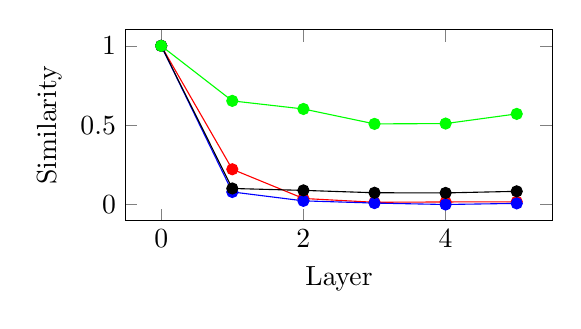
\begin{tikzpicture}
\begin{axis}[
	height=4cm,
	width=7cm,
	xlabel={Layer},
	ylabel={Similarity},
%	xmin=40, xmax=80,
%	ymin=0,  ymax=68,
	legend columns=2,
    legend to name=sanity_leg,
    legend style={font=\footnotesize}
]
	\addplot[mark=*,red] coordinates{(0,1.0)(1,0.222)(2,0.038)(3,0.014)(4,0.016)(5,0.017)};   \leg{Rank Correl (No Abs)}
	\addplot[mark=*,blue] coordinates{(0,1.0)(1,0.079)(2,0.023)(3,0.009)(4,0.000)(5,0.007)}; \leg{Rank Correl (Abs)}
	\addplot[mark=*,black] coordinates{(0,1.0)(1,0.101)(2,0.089)(3,0.074)(4,0.073)(5,0.083)}; \leg{HOGs similarity}
	\addplot[mark=*,green] coordinates{(0,1.0)(1,0.653)(2,0.602)(3,0.508)(4,0.510)(5,0.571)}; \leg{SSIM}
\end{axis}
\end{tikzpicture}
}
\caption{\emph{Sanity check} of Opti-CAM on $1,000$ images of ImageNet validation set using ResNet50. Similarity between saliency maps by original and randomized network, where layers are progressively replaced by random ones.}
\label{fig:sanity}
\end{figure}
%------------------------------------------------------------------------------

%------------------------------------------------------------------------------
\begin{figure}[htpb]
\newcommand{\sizeP}{.12}
\newcommand{\sizeS}{.15}
\newcommand{\hh}{.175\textwidth}
\newcommand{\ww}{.200\textwidth}
\centering
\small
\setlength{\tabcolsep}{3pt}
\begin{tabular}{cccccc}
Original & layer 1 & layer 2 & layer 3 & layer 4 & layer 5 \\
\fig[\sizeS]{sanityC/ILSVRC2012_val_00000001JPEG_0_Smap.png} &
\fig[\sizeS]{sanityC/ILSVRC2012_val_00000001JPEG_1_Smap.png} &
\fig[\sizeS]{sanityC/ILSVRC2012_val_00000001JPEG_2_Smap.png} &
\fig[\sizeS]{sanityC/ILSVRC2012_val_00000001JPEG_3_Smap.png} &
\fig[\sizeS]{sanityC/ILSVRC2012_val_00000001JPEG_4_Smap.png} &
\fig[\sizeS]{sanityC/ILSVRC2012_val_00000001JPEG_6_Smap.png} \\
\fig[\sizeS]{sanityC/ILSVRC2012_val_00000002JPEG_0_Smap.png} &
\fig[\sizeS]{sanityC/ILSVRC2012_val_00000002JPEG_1_Smap.png} &
\fig[\sizeS]{sanityC/ILSVRC2012_val_00000002JPEG_2_Smap.png} &
\fig[\sizeS]{sanityC/ILSVRC2012_val_00000002JPEG_3_Smap.png} &
\fig[\sizeS]{sanityC/ILSVRC2012_val_00000002JPEG_4_Smap.png} &
\fig[\sizeS]{sanityC/ILSVRC2012_val_00000002JPEG_6_Smap.png} \\
\end{tabular}
\caption{\emph{Sanity check visualization} of Opti-CAM on two images of ImageNet validation set using ResNet50. First column: Opti-CAM saliency maps for the original network; remaining columns: Opti-CAM saliency maps where layers are progressively replaced by random ones.}
\label{fig:sanity-vis}
\end{figure}
%------------------------------------------------------------------------------

\section{Sanity check}
\label{sec:sanity-check}

We use the model parameter randomization test proposed by~\citep{adebayosanity}. This test compares the saliency maps generated by a trained model with the ones generated by a partially randomly initialized network of the same architecture. In particular, we choose 5 layers of ResNet50 and we progressively replace them by random ones so that we have 6 different models with different amount of random parameters. The saliency maps are generated for the small subset of ImageNet validation set, as in the ablation study.

Following~\citep{adebayosanity}, we compute a number of similarity metrics between these saliency maps generated by the original and the randomized network, including Rank Correlation with/without absolute values, HOGs similarity, and SSIM. The results are shown in \autoref{fig:sanity} (saliency map similarity measurements) and \autoref{fig:sanity-vis} (saliency map visualizations). Our method passes the sanity check, as it is very sensitive to changes in the model parameters. \modify{We also use model parameter randomization test and train a ResNet50 with randomly permuted labels following the training recipes from the pytorch models\footnote{\url{https://github.com/pytorch/vision/tree/main/references/classification}}. The SSIM similarity is $0.013$, which shows that Opti-CAM is sensitive to the relationship between instances and labels.}

%------------------------------------------------------------------------------
\begin{table}[htbp]
\centering
\footnotesize
\setlength{\tabcolsep}{4pt}
\renewcommand{\arraystretch}{0.8}
\begin{tabular}{lrrrr|rrrr} \toprule
\mr{2}{\Th{Method}}                                & \mc{4}{\Th{ResNet50}} & \mc{4}{\Th{VGG16}} \\ \cmidrule{2-9}
                                                   & {$\AD\!\downarrow$} & {$\AG\!\uparrow$} & {$\AI\!\uparrow$} & \mc{1}{T} & {$\AD\!\downarrow$} & {$\AG\!\uparrow$} & {$\AI\!\uparrow$} & \mc{1}{T} \\ \midrule
Fake-CAM~\citep{poppi2021revisiting}               &0.9&0.7&47.4&0.00&0.5&0.3&47.7&0.00  \\ \midrule
Grad-CAM~\citep{selvaraju2017grad}       & 36.4      &5.5& 27.0      &0.03     & 41.6     &3.3 & 25.2       &0.02     \\
Grad-CAM++~\cite{chattopadhay2018grad}    & 37.6    & 4.9 & 24.0       &0.04    & 46.3     &2.0 & 19.0        &0.02    \\
Score-CAM~\citep{wang2020score}           & 28.8     &8.8 & 33.6       &20.47& 39.3    & 3.5 & 24.6       &3.08     \\
Ablation-CAM~\citep{ramaswamy2020ablation}   & 36.6      &5.1& 25.6      &18.49 & 41.8     & 2.9& 24.0       &2.95    \\
XGrad-CAM~\citep{fu2020axiom}            & 36.4     &5.5 & 27.0       &0.03   & 40.6     &3.4 & 25.8       &0.02   \\
Layer-CAM~\citep{jiang2021layercam} &42.6&4.2&19.2&0.02&82.1&0.3&6.9&0.01   \\
ExPerturbation~\citep{fong2019understanding} &51.2&6.9&26.1&15.67&50.1&4.4&24.5&9.10  \\
\rowcolor{cyan!10}
Opti-CAM (ours)                          &\tb{2.0}&\tb{49.4}&\tb{91.2}&3.94&\tb{1.5}&\tb{52.7}&\tb{92.1}&3.95\\
\bottomrule
\end{tabular}
% \vspace{6pt}
\caption{
\emph{Classification metrics} on ImageNet validation set, without input normalization. AD/AI: average drop/increase~\citep{chattopadhay2018grad}; $\AG$: average gain (ours); $\downarrow$ / $\uparrow$: lower / higher is better. T: Average time (sec) per batch of 8 images. Bold: best, excluding Fake-CAM.}
\label{tab:norm-imagenet}
\end{table}
%------------------------------------------------------------------------------

\section{Results without input normalization}
\label{sec:without-norm}

It is standard that images are normalized to zero mean and unit standard deviation before feeding them to a network, because this is how networks are trained. For example, for ImageNet images, we subtract the mean vector $[0.485,0.456,0.406]$ and divide channel-wise by standard deviation $[0.229,0.224,0.225]$. By doing so however, we cannot reproduce the results published for several baseline methods; rather, all results are improved dramatically. We can obtain results similar to published ones by \emph{not} normalizing, thus we speculate that authors of related work do not normalize images. This is also suggested by our attempts to communicate with the authors.

We believe normalization is important and we include it in all our experiments. For reference and to allow for comparison with published results, we provide results without normalization in \autoref{tab:norm-imagenet} that correspond to \autoref{tab:imagenet-cnn}. Finally, code is provided to allow for the reproduction and verification of our results.

% %------------------------------------------------------------------------------
% % \input{tex/IN_n_chest_n_kvasir_vgg16}
% \begin{figure*}
% \vspace{-0.4cm}
\newcommand{\sizeS}{.12}
\centering
\footnotesize
\setlength{\tabcolsep}{1pt}
\begin{tabular}{c cccc cccc}
     & \mc{4}{VGG16} & \mc{4}{ResNet50}\\
	Input image  &  Grad-CAM  & G-CAM++ & Score-CAM & Opti-CAM  &Grad-CAM  & G-CAM++ & Score-CAM & Opti-CAM \\
	\fig[\sizeS]{medical/chest_Resnet50_GradCAM_0_0img.png} &
	\fig[\sizeS]{medical/chest_VGG16_GradCAM_0_0vis.png} &\fig[\sizeS]{medical/chest_Resnet50_GradCAM_0_0vis.png} &
	\fig[\sizeS]{medical/chest_VGG16_GradCAMPlusPlus_0_0vis.png} &\fig[\sizeS]{medical/chest_Resnet50_GradCAMPlusPlus_0_0vis.png} &
	\fig[\sizeS]{medical/chest_VGG16_ScoreCAM_0_0vis.png} &\fig[\sizeS]{medical/chest_Resnet50_ScoreCAM_0_0vis.png} &
	\fig[\sizeS]{medical/chest_VGG16_OptCAM_0_0vis.png} & \fig[\sizeS]{medical/chest_Resnet50_OptCAM_0_0vis.png} \\
 
\fig[\sizeS]{medical/chest_Resnet50_GradCAM_0_1img.png} &
	\fig[\sizeS]{medical/chest_VGG16_GradCAM_0_1vis.png} &\fig[\sizeS]{medical/chest_Resnet50_GradCAM_0_1vis.png} &
	\fig[\sizeS]{medical/chest_VGG16_GradCAMPlusPlus_0_1vis.png} &\fig[\sizeS]{medical/chest_Resnet50_GradCAMPlusPlus_0_1vis.png} &
	\fig[\sizeS]{medical/chest_VGG16_ScoreCAM_0_1vis.png} &\fig[\sizeS]{medical/chest_Resnet50_ScoreCAM_0_1vis.png} &
	\fig[\sizeS]{medical/chest_VGG16_OptCAM_0_1vis.png} & \fig[\sizeS]{medical/chest_Resnet50_OptCAM_0_1vis.png} \\
 
\fig[\sizeS]{medical/chest_Resnet50_GradCAM_0_2img.png} &
	\fig[\sizeS]{medical/chest_VGG16_GradCAM_0_2vis.png} &\fig[\sizeS]{medical/chest_Resnet50_GradCAM_0_2vis.png} &
	\fig[\sizeS]{medical/chest_VGG16_GradCAMPlusPlus_0_2vis.png} &\fig[\sizeS]{medical/chest_Resnet50_GradCAMPlusPlus_0_2vis.png} &
	\fig[\sizeS]{medical/chest_VGG16_ScoreCAM_0_2vis.png} &\fig[\sizeS]{medical/chest_Resnet50_ScoreCAM_0_2vis.png} &
	\fig[\sizeS]{medical/chest_VGG16_OptCAM_0_2vis.png} & \fig[\sizeS]{medical/chest_Resnet50_OptCAM_0_2vis.png} \\
 
\fig[\sizeS]{medical/chest_Resnet50_GradCAM_0_3img.png} &
	\fig[\sizeS]{medical/chest_VGG16_GradCAM_0_3vis.png} &\fig[\sizeS]{medical/chest_Resnet50_GradCAM_0_3vis.png} &
	\fig[\sizeS]{medical/chest_VGG16_GradCAMPlusPlus_0_3vis.png} &\fig[\sizeS]{medical/chest_Resnet50_GradCAMPlusPlus_0_3vis.png} &
	\fig[\sizeS]{medical/chest_VGG16_ScoreCAM_0_3vis.png} &\fig[\sizeS]{medical/chest_Resnet50_ScoreCAM_0_3vis.png} &
	\fig[\sizeS]{medical/chest_VGG16_OptCAM_0_3vis.png} & \fig[\sizeS]{medical/chest_Resnet50_OptCAM_0_3vis.png} \\
 
	\fig[\sizeS]{medical/chest_Resnet50_GradCAM_1_4img.png} &
	\fig[\sizeS]{medical/chest_VGG16_GradCAM_1_4vis.png} &\fig[\sizeS]{medical/chest_Resnet50_GradCAM_1_4vis.png} &
	\fig[\sizeS]{medical/chest_VGG16_GradCAMPlusPlus_1_4vis.png} &\fig[\sizeS]{medical/chest_Resnet50_GradCAMPlusPlus_1_4vis.png} &
	\fig[\sizeS]{medical/chest_VGG16_ScoreCAM_1_4vis.png} &\fig[\sizeS]{medical/chest_Resnet50_ScoreCAM_1_4vis.png} &
	\fig[\sizeS]{medical/chest_VGG16_OptCAM_1_4vis.png} & \fig[\sizeS]{medical/chest_Resnet50_OptCAM_1_4vis.png} \\

 \fig[\sizeS]{medical/chest_Resnet50_GradCAM_1_5img.png} &
	\fig[\sizeS]{medical/chest_VGG16_GradCAM_1_5vis.png} &\fig[\sizeS]{medical/chest_Resnet50_GradCAM_1_5vis.png} &
	\fig[\sizeS]{medical/chest_VGG16_GradCAMPlusPlus_1_5vis.png} &\fig[\sizeS]{medical/chest_Resnet50_GradCAMPlusPlus_1_5vis.png} &
	\fig[\sizeS]{medical/chest_VGG16_ScoreCAM_1_5vis.png} &\fig[\sizeS]{medical/chest_Resnet50_ScoreCAM_1_5vis.png} &
	\fig[\sizeS]{medical/chest_VGG16_OptCAM_1_5vis.png} & \fig[\sizeS]{medical/chest_Resnet50_OptCAM_1_5vis.png} \\

 \fig[\sizeS]{medical/chest_Resnet50_GradCAM_1_6img.png} &
	\fig[\sizeS]{medical/chest_VGG16_GradCAM_1_6vis.png} &\fig[\sizeS]{medical/chest_Resnet50_GradCAM_1_6vis.png} &
	\fig[\sizeS]{medical/chest_VGG16_GradCAMPlusPlus_1_6vis.png} &\fig[\sizeS]{medical/chest_Resnet50_GradCAMPlusPlus_1_6vis.png} &
	\fig[\sizeS]{medical/chest_VGG16_ScoreCAM_1_6vis.png} &\fig[\sizeS]{medical/chest_Resnet50_ScoreCAM_1_6vis.png} &
	\fig[\sizeS]{medical/chest_VGG16_OptCAM_1_6vis.png} & \fig[\sizeS]{medical/chest_Resnet50_OptCAM_1_6vis.png} \\

 \fig[\sizeS]{medical/chest_Resnet50_GradCAM_1_7img.png} &
	\fig[\sizeS]{medical/chest_VGG16_GradCAM_1_7vis.png} &\fig[\sizeS]{medical/chest_Resnet50_GradCAM_1_7vis.png} &
	\fig[\sizeS]{medical/chest_VGG16_GradCAMPlusPlus_1_7vis.png} &\fig[\sizeS]{medical/chest_Resnet50_GradCAMPlusPlus_1_7vis.png} &
	\fig[\sizeS]{medical/chest_VGG16_ScoreCAM_1_7vis.png} &\fig[\sizeS]{medical/chest_Resnet50_ScoreCAM_1_7vis.png} &
	\fig[\sizeS]{medical/chest_VGG16_OptCAM_1_7vis.png} & \fig[\sizeS]{medical/chest_Resnet50_OptCAM_1_7vis.png} \\
\end{tabular}
\caption{Saliency maps obtained from Chest X-ray images.}
\label{fig:vis-chest-resnet}
% \vspace{-0.8cm}
\end{figure*}

% 
\begin{figure*}
\newcommand{\sizeS}{.12}
\centering
\footnotesize
\setlength{\tabcolsep}{1pt}
\begin{tabular}{c cccc cccc}
     & \mc{4}{VGG16} & \mc{4}{ResNet50}\\
	Input image  &  Grad-CAM  & G-CAM++ & Score-CAM & Opti-CAM  &Grad-CAM  & G-CAM++ & Score-CAM & Opti-CAM \\
	\fig[\sizeS]{medical/kvasir_Resnet50_GradCAM_0_img.png} &
	\fig[\sizeS]{medical/kvasir_VGG16_GradCAM_0_vis.png} &
	\fig[\sizeS]{medical/kvasir_VGG16_GradCAMPlusPlus_0_vis.png} &
	\fig[\sizeS]{medical/kvasir_VGG16_ScoreCAM_0_vis.png} &
	\fig[\sizeS]{medical/kvasir_VGG16_OptCAM_0_vis.png} &
		\fig[\sizeS]{medical/kvasir_Resnet50_GradCAM_0_vis.png} &
	\fig[\sizeS]{medical/kvasir_Resnet50_GradCAMPlusPlus_0_vis.png} &
	\fig[\sizeS]{medical/kvasir_Resnet50_ScoreCAM_0_vis.png} &
	\fig[\sizeS]{medical/kvasir_Resnet50_OptCAM_0_vis.png}
	\\
	\fig[\sizeS]{medical/kvasir_VGG16_GradCAM_1_img.png} &
	\fig[\sizeS]{medical/kvasir_VGG16_GradCAM_1_vis.png} &
	\fig[\sizeS]{medical/kvasir_VGG16_GradCAMPlusPlus_1_vis.png} &
	\fig[\sizeS]{medical/kvasir_VGG16_ScoreCAM_1_vis.png} &
	\fig[\sizeS]{medical/kvasir_VGG16_OptCAM_1_vis.png} &
	\fig[\sizeS]{medical/kvasir_Resnet50_GradCAM_1_vis.png} &
	\fig[\sizeS]{medical/kvasir_Resnet50_GradCAMPlusPlus_1_vis.png} &
	\fig[\sizeS]{medical/kvasir_Resnet50_ScoreCAM_1_vis.png} &
	\fig[\sizeS]{medical/kvasir_Resnet50_OptCAM_1_vis.png} 
	
	\\
	\fig[\sizeS]{medical/kvasir_VGG16_GradCAM_2_img.png} &
	\fig[\sizeS]{medical/kvasir_VGG16_GradCAM_2_vis.png} &
	\fig[\sizeS]{medical/kvasir_VGG16_GradCAMPlusPlus_2_vis.png} &
	\fig[\sizeS]{medical/kvasir_VGG16_ScoreCAM_2_vis.png} &
	\fig[\sizeS]{medical/kvasir_VGG16_OptCAM_2_vis.png} &
	\fig[\sizeS]{medical/kvasir_Resnet50_GradCAM_2_vis.png} &
	\fig[\sizeS]{medical/kvasir_Resnet50_GradCAMPlusPlus_2_vis.png} &
	\fig[\sizeS]{medical/kvasir_Resnet50_ScoreCAM_2_vis.png} &
	\fig[\sizeS]{medical/kvasir_Resnet50_OptCAM_2_vis.png}\\
	
	
	\fig[\sizeS]{medical/kvasir_Resnet50_GradCAM_3_img.png} &
	\fig[\sizeS]{medical/kvasir_VGG16_GradCAM_3_vis.png} &
	\fig[\sizeS]{medical/kvasir_VGG16_GradCAMPlusPlus_3_vis.png} &
	\fig[\sizeS]{medical/kvasir_VGG16_ScoreCAM_3_vis.png} &
	\fig[\sizeS]{medical/kvasir_VGG16_OptCAM_3_vis.png} &
	\fig[\sizeS]{medical/kvasir_Resnet50_GradCAM_3_vis.png} &
	\fig[\sizeS]{medical/kvasir_Resnet50_GradCAMPlusPlus_3_vis.png} &
	\fig[\sizeS]{medical/kvasir_Resnet50_ScoreCAM_3_vis.png} &
	\fig[\sizeS]{medical/kvasir_Resnet50_OptCAM_3_vis.png}
	\\
	\fig[\sizeS]{medical/kvasir_Resnet50_GradCAM_4_img.png} &
	\fig[\sizeS]{medical/kvasir_VGG16_GradCAM_4_vis.png} &
	\fig[\sizeS]{medical/kvasir_VGG16_GradCAMPlusPlus_4_vis.png} &
	\fig[\sizeS]{medical/kvasir_VGG16_ScoreCAM_4_vis.png} &
	\fig[\sizeS]{medical/kvasir_VGG16_OptCAM_4_vis.png} &
	\fig[\sizeS]{medical/kvasir_Resnet50_GradCAM_4_vis.png} &
	\fig[\sizeS]{medical/kvasir_Resnet50_GradCAMPlusPlus_4_vis.png} &
	\fig[\sizeS]{medical/kvasir_Resnet50_ScoreCAM_4_vis.png} &
	\fig[\sizeS]{medical/kvasir_Resnet50_OptCAM_4_vis.png}
	\\
	\fig[\sizeS]{medical/kvasir_Resnet50_GradCAM_5_img.png} &
	\fig[\sizeS]{medical/kvasir_VGG16_GradCAM_5_vis.png} &
	\fig[\sizeS]{medical/kvasir_VGG16_GradCAMPlusPlus_5_vis.png} &
	\fig[\sizeS]{medical/kvasir_VGG16_ScoreCAM_5_vis.png} &
	\fig[\sizeS]{medical/kvasir_VGG16_OptCAM_5_vis.png}  &
	\fig[\sizeS]{medical/kvasir_Resnet50_GradCAM_5_vis.png} &
	\fig[\sizeS]{medical/kvasir_Resnet50_GradCAMPlusPlus_5_vis.png} &
	\fig[\sizeS]{medical/kvasir_Resnet50_ScoreCAM_5_vis.png} &
	\fig[\sizeS]{medical/kvasir_Resnet50_OptCAM_5_vis.png} 
	\\
	\fig[\sizeS]{medical/kvasir_Resnet50_GradCAM_6_img.png} &
	\fig[\sizeS]{medical/kvasir_VGG16_GradCAM_6_vis.png} &
	\fig[\sizeS]{medical/kvasir_VGG16_GradCAMPlusPlus_6_vis.png} &
	\fig[\sizeS]{medical/kvasir_VGG16_ScoreCAM_6_vis.png} &
	\fig[\sizeS]{medical/kvasir_VGG16_OptCAM_6_vis.png} &
	\fig[\sizeS]{medical/kvasir_Resnet50_GradCAM_6_vis.png} &
	\fig[\sizeS]{medical/kvasir_Resnet50_GradCAMPlusPlus_6_vis.png} &
	\fig[\sizeS]{medical/kvasir_Resnet50_ScoreCAM_6_vis.png} &
	\fig[\sizeS]{medical/kvasir_Resnet50_OptCAM_6_vis.png} 
	\\
	\fig[\sizeS]{medical/kvasir_Resnet50_GradCAM_7_img.png} &
	\fig[\sizeS]{medical/kvasir_VGG16_GradCAM_7_vis.png} &
	\fig[\sizeS]{medical/kvasir_VGG16_GradCAMPlusPlus_7_vis.png} &
	\fig[\sizeS]{medical/kvasir_VGG16_ScoreCAM_7_vis.png} &
	\fig[\sizeS]{medical/kvasir_VGG16_OptCAM_7_vis.png} &
	\fig[\sizeS]{medical/kvasir_Resnet50_GradCAM_7_vis.png} &
	\fig[\sizeS]{medical/kvasir_Resnet50_GradCAMPlusPlus_7_vis.png} &
	\fig[\sizeS]{medical/kvasir_Resnet50_ScoreCAM_7_vis.png} &
	\fig[\sizeS]{medical/kvasir_Resnet50_OptCAM_7_vis.png} \\
\end{tabular}
\caption{Saliency maps obtained for KVASIR images.}
\label{fig:vis-kvasir-resnet}
\end{figure*}



% \input{tex/show_image_vgg}
% \begin{figure*}[t]
\newcommand{\sizeP}{.14}
\newcommand{\sizeS}{.14}
\newcommand{\hh}{.175\textwidth}
\newcommand{\ww}{.200\textwidth}
\scriptsize
\centering
\setlength{\tabcolsep}{3pt}
\begin{tabular}{ccccccc}
	Input image  &  Grad-CAM  & G-CAM++ & Score-CAM & Ablation-CAM & XG-CAM & Opti-CAM (ours) \\
        \includegraphics[trim={12mm 14mm 12mm 14mm},clip, width=\sizeP\textwidth]{fig/visual/ILSVRC2012_val_00000089.JPEG}&
	\fig[\sizeS]{visual/Resnet50_GradCAM_ILSVRC2012_val_00000089.png} &
	\fig[\sizeS]{visual/Resnet50_GradCAMPlusPlus_ILSVRC2012_val_00000089.png} &
	\fig[\sizeS]{visual/Resnet50_ScoreCAM_ILSVRC2012_val_00000089.png} &
	\fig[\sizeS]{visual/Resnet50_AblationCAM_ILSVRC2012_val_00000089.png} &
	\fig[\sizeS]{visual/Resnet50_XGradCAM_ILSVRC2012_val_00000089.png} & 
	\fig[\sizeS]{visual/Resnet50_OptCAM_ILSVRC2012_val_00000089.png}  \\
	Cellphone &&&&&& \\
	\fig[\sizeS]{visual/ILSVRC2012_val_00000748.png}&
	\fig[\sizeS]{visual/Resnet50_GradCAM_ILSVRC2012_val_00000748.png} &
	\fig[\sizeS]{visual/Resnet50_GradCAMPlusPlus_ILSVRC2012_val_00000748.png} &
	\fig[\sizeS]{visual/Resnet50_ScoreCAM_ILSVRC2012_val_00000748.png} &
	\fig[\sizeS]{visual/Resnet50_AblationCAM_ILSVRC2012_val_00000748.png} &
	\fig[\sizeS]{visual/Resnet50_XGradCAM_ILSVRC2012_val_00000748.png} & 
	\fig[\sizeS]{visual/Resnet50_OptCAM_ILSVRC2012_val_00000748.png}  \\
	Miniature Schnauzer &&&&&& \\
	\includegraphics[trim={2mm 3mm 6mm 1mm},clip, width=\sizeP\textwidth]{fig/visual/ILSVRC2012_val_00000769.JPEG}&
	\fig[\sizeS]{visual/Resnet50_GradCAM_ILSVRC2012_val_00000769.png} &
	\fig[\sizeS]{visual/Resnet50_GradCAMPlusPlus_ILSVRC2012_val_00000769.png} &
	\fig[\sizeS]{visual/Resnet50_ScoreCAM_ILSVRC2012_val_00000769.png} &
	\fig[\sizeS]{visual/Resnet50_AblationCAM_ILSVRC2012_val_00000769.png} &
	\fig[\sizeS]{visual/Resnet50_XGradCAM_ILSVRC2012_val_00000769.png} & 
	\fig[\sizeS]{visual/Resnet50_OptCAM_ILSVRC2012_val_00000769.png}  \\
	Face Powder &&&&&& \\
	\includegraphics[trim={2mm 6mm 2mm 6mm},clip, width=\sizeP\textwidth]{fig/visual/ILSVRC2012_val_00000782.JPEG}&
	\fig[\sizeS]{visual/Resnet50_GradCAM_ILSVRC2012_val_00000782.png} &
	\fig[\sizeS]{visual/Resnet50_GradCAMPlusPlus_ILSVRC2012_val_00000782.png} &
	\fig[\sizeS]{visual/Resnet50_ScoreCAM_ILSVRC2012_val_00000782.png} &
	\fig[\sizeS]{visual/Resnet50_AblationCAM_ILSVRC2012_val_00000782.png} &
	\fig[\sizeS]{visual/Resnet50_XGradCAM_ILSVRC2012_val_00000782.png} & 
	\fig[\sizeS]{visual/Resnet50_OptCAM_ILSVRC2012_val_00000782.png}  \\
	Chocolate Sauce &&&&&& \\
	\fig[\sizeS]{visual/ILSVRC2012_val_00001113.png}&
	\fig[\sizeS]{visual/Resnet50_GradCAM_ILSVRC2012_val_00001113.png} &
	\fig[\sizeS]{visual/Resnet50_GradCAMPlusPlus_ILSVRC2012_val_00001113.png} &
	\fig[\sizeS]{visual/Resnet50_ScoreCAM_ILSVRC2012_val_00001113.png} &
	\fig[\sizeS]{visual/Resnet50_AblationCAM_ILSVRC2012_val_00001113.png} &
	\fig[\sizeS]{visual/Resnet50_XGradCAM_ILSVRC2012_val_00001113.png} & 
	\fig[\sizeS]{visual/Resnet50_OptCAM_ILSVRC2012_val_00001113.png}  \\
	Komondor &&&&&& \\
 \includegraphics[trim={14mm 16mm 14mm 12mm},clip, width=\sizeP\textwidth]{fig/visual/ILSVRC2012_val_00001345.JPEG}&
	\fig[\sizeS]{visual/Resnet50_GradCAM_ILSVRC2012_val_00001345.png} &
	\fig[\sizeS]{visual/Resnet50_GradCAMPlusPlus_ILSVRC2012_val_00001345.png} &
	\fig[\sizeS]{visual/Resnet50_ScoreCAM_ILSVRC2012_val_00001345.png} &
	\fig[\sizeS]{visual/Resnet50_AblationCAM_ILSVRC2012_val_00001345.png} &
	\fig[\sizeS]{visual/Resnet50_XGradCAM_ILSVRC2012_val_00001345.png} & 
	\fig[\sizeS]{visual/Resnet50_OptCAM_ILSVRC2012_val_00001345.png}  \\
	Quill &&&&&& \\
 \includegraphics[trim={5mm 14mm 5mm 14mm},clip, width=\sizeP\textwidth]{fig/visual/ILSVRC2012_val_00001529.JPEG}&
	\fig[\sizeS]{visual/Resnet50_GradCAM_ILSVRC2012_val_00001529.png} &
	\fig[\sizeS]{visual/Resnet50_GradCAMPlusPlus_ILSVRC2012_val_00001529.png} &
	\fig[\sizeS]{visual/Resnet50_ScoreCAM_ILSVRC2012_val_00001529.png} &
	\fig[\sizeS]{visual/Resnet50_AblationCAM_ILSVRC2012_val_00001529.png} &
	\fig[\sizeS]{visual/Resnet50_XGradCAM_ILSVRC2012_val_00001529.png} & 
	\fig[\sizeS]{visual/Resnet50_OptCAM_ILSVRC2012_val_00001529.png}  \\
	Longicorn &&&&&& \\
 \includegraphics[trim={8mm 1mm 8mm 1mm},clip, width=\sizeP\textwidth]{fig/visual/ILSVRC2012_val_00001635.JPEG}&
	\fig[\sizeS]{visual/Resnet50_GradCAM_ILSVRC2012_val_00001635.png} &
	\fig[\sizeS]{visual/Resnet50_GradCAMPlusPlus_ILSVRC2012_val_00001635.png} &
	\fig[\sizeS]{visual/Resnet50_ScoreCAM_ILSVRC2012_val_00001635.png} &
	\fig[\sizeS]{visual/Resnet50_AblationCAM_ILSVRC2012_val_00001635.png} &
	\fig[\sizeS]{visual/Resnet50_XGradCAM_ILSVRC2012_val_00001635.png} & 
	\fig[\sizeS]{visual/Resnet50_OptCAM_ILSVRC2012_val_00001635.png}  \\
	Slide Rule &&&&&& \\
\end{tabular}
% \vspace{5pt}
\caption{Saliency maps obtained from ImageNet example images using different methods on ResNet50.}
\label{fig:imagenet-vis-more-res}
\end{figure*}

% % \begin{figure*}[t]
\newcommand{\sizeP}{.12}
\newcommand{\sizeS}{.12}
\newcommand{\hh}{.175\textwidth}
\newcommand{\ww}{.200\textwidth}
\tiny
\centering
\setlength{\tabcolsep}{1pt}
\begin{tabular}{cccccccc}
	Input image  &  Grad-CAM  & G-CAM++ & Score-CAM & XG-CAM & Raw Att. & Rollout & Opti-CAM (ours) \\
        \includegraphics[trim={12mm 14mm 12mm 14mm},clip, width=\sizeP\textwidth]{fig/visual/ILSVRC2012_val_00000089.JPEG}&
	\fig[\sizeS]{visual/ViT_GradCAM_ILSVRC2012_val_00000089.png} &
	\fig[\sizeS]{visual/ViT_GradCAMPlusPlus_ILSVRC2012_val_00000089.png} &
	\fig[\sizeS]{visual/ViT_ScoreCAM_ILSVRC2012_val_00000089.png} &
	\fig[\sizeS]{visual/ViT_XGradCAM_ILSVRC2012_val_00000089.png} & 
        \fig[\sizeS]{visual/ViT_RawAttention_ILSVRC2012_val_00000089.png} &
        \fig[\sizeS]{visual/ViT_RolloutMean_ILSVRC2012_val_00000089.png} &
	\fig[\sizeS]{visual/ViT_OptiCAM_ILSVRC2012_val_00000089.png}  \\
	Cellphone &&&&&& \\
	\fig[\sizeS]{visual/ILSVRC2012_val_00000748.png}&
	\fig[\sizeS]{visual/ViT_GradCAM_ILSVRC2012_val_00000748.png} &
	\fig[\sizeS]{visual/ViT_GradCAMPlusPlus_ILSVRC2012_val_00000748.png} &
	\fig[\sizeS]{visual/ViT_ScoreCAM_ILSVRC2012_val_00000748.png} &
	\fig[\sizeS]{visual/ViT_XGradCAM_ILSVRC2012_val_00000748.png} & 
        \fig[\sizeS]{visual/ViT_RawAttention_ILSVRC2012_val_00000748.png} &
        \fig[\sizeS]{visual/ViT_RolloutMean_ILSVRC2012_val_00000748.png} &
	\fig[\sizeS]{visual/ViT_OptiCAM_ILSVRC2012_val_00000748.png}  \\
	Miniature Schnauzer &&&&&& \\
	\includegraphics[trim={2mm 3mm 6mm 1mm},clip, width=\sizeP\textwidth]{fig/visual/ILSVRC2012_val_00000769.JPEG}&
	\fig[\sizeS]{visual/ViT_GradCAM_ILSVRC2012_val_00000769.png} &
	\fig[\sizeS]{visual/ViT_GradCAMPlusPlus_ILSVRC2012_val_00000769.png} &
	\fig[\sizeS]{visual/ViT_ScoreCAM_ILSVRC2012_val_00000769.png} &
	\fig[\sizeS]{visual/ViT_XGradCAM_ILSVRC2012_val_00000769.png} & 
        \fig[\sizeS]{visual/ViT_RawAttention_ILSVRC2012_val_00000769.png} &
        \fig[\sizeS]{visual/ViT_RolloutMean_ILSVRC2012_val_00000769.png} &
	\fig[\sizeS]{visual/ViT_OptiCAM_ILSVRC2012_val_00000769.png}  \\
	Face Powder &&&&&& \\
	\includegraphics[trim={2mm 6mm 2mm 6mm},clip, width=\sizeP\textwidth]{fig/visual/ILSVRC2012_val_00000782.JPEG}&
	\fig[\sizeS]{visual/ViT_GradCAM_ILSVRC2012_val_00000782.png} &
	\fig[\sizeS]{visual/ViT_GradCAMPlusPlus_ILSVRC2012_val_00000782.png} &
	\fig[\sizeS]{visual/ViT_ScoreCAM_ILSVRC2012_val_00000782.png} &
	\fig[\sizeS]{visual/ViT_XGradCAM_ILSVRC2012_val_00000782.png} & 
        \fig[\sizeS]{visual/ViT_RawAttention_ILSVRC2012_val_00000782.png} &
        \fig[\sizeS]{visual/ViT_RolloutMean_ILSVRC2012_val_00000782.png} &
	\fig[\sizeS]{visual/ViT_OptiCAM_ILSVRC2012_val_00000782.png}  \\
	Chocolate Sauce &&&&&& \\
	\fig[\sizeS]{visual/ILSVRC2012_val_00001113.png}&
	\fig[\sizeS]{visual/ViT_GradCAM_ILSVRC2012_val_00001113.png} &
	\fig[\sizeS]{visual/ViT_GradCAMPlusPlus_ILSVRC2012_val_00001113.png} &
	\fig[\sizeS]{visual/ViT_ScoreCAM_ILSVRC2012_val_00001113.png} &
	\fig[\sizeS]{visual/ViT_XGradCAM_ILSVRC2012_val_00001113.png} & 
        \fig[\sizeS]{visual/ViT_RawAttention_ILSVRC2012_val_00001113.png} &
        \fig[\sizeS]{visual/ViT_RolloutMean_ILSVRC2012_val_00001113.png} &
	\fig[\sizeS]{visual/ViT_OptiCAM_ILSVRC2012_val_00001113.png}  \\
	Komondor &&&&&& \\
 \includegraphics[trim={14mm 16mm 14mm 12mm},clip, width=\sizeP\textwidth]{fig/visual/ILSVRC2012_val_00001345.JPEG}&
	\fig[\sizeS]{visual/ViT_GradCAM_ILSVRC2012_val_00001345.png} &
	\fig[\sizeS]{visual/ViT_GradCAMPlusPlus_ILSVRC2012_val_00001345.png} &
	\fig[\sizeS]{visual/ViT_ScoreCAM_ILSVRC2012_val_00001345.png} &
	\fig[\sizeS]{visual/ViT_XGradCAM_ILSVRC2012_val_00001345.png} & 
        \fig[\sizeS]{visual/ViT_RawAttention_ILSVRC2012_val_00001345.png} &
        \fig[\sizeS]{visual/ViT_RolloutMean_ILSVRC2012_val_00001345.png} &
	\fig[\sizeS]{visual/ViT_OptiCAM_ILSVRC2012_val_00001345.png}  \\
	Quill &&&&&& \\
 \includegraphics[trim={5mm 14mm 5mm 14mm},clip, width=\sizeP\textwidth]{fig/visual/ILSVRC2012_val_00001529.JPEG}&
	\fig[\sizeS]{visual/ViT_GradCAM_ILSVRC2012_val_00001529.png} &
	\fig[\sizeS]{visual/ViT_GradCAMPlusPlus_ILSVRC2012_val_00001529.png} &
	\fig[\sizeS]{visual/ViT_ScoreCAM_ILSVRC2012_val_00001529.png} &
	\fig[\sizeS]{visual/ViT_XGradCAM_ILSVRC2012_val_00001529.png} & 
        \fig[\sizeS]{visual/ViT_RawAttention_ILSVRC2012_val_00001529.png} &
        \fig[\sizeS]{visual/ViT_RolloutMean_ILSVRC2012_val_00001529.png} &
	\fig[\sizeS]{visual/ViT_OptiCAM_ILSVRC2012_val_00001529.png}  \\
	Longicorn &&&&&& \\
 \includegraphics[trim={8mm 1mm 8mm 1mm},clip, width=\sizeP\textwidth]{fig/visual/ILSVRC2012_val_00001635.JPEG}&
	\fig[\sizeS]{visual/ViT_GradCAM_ILSVRC2012_val_00001635.png} &
	\fig[\sizeS]{visual/ViT_GradCAMPlusPlus_ILSVRC2012_val_00001635.png} &
	\fig[\sizeS]{visual/ViT_ScoreCAM_ILSVRC2012_val_00001635.png} &
	\fig[\sizeS]{visual/ViT_XGradCAM_ILSVRC2012_val_00001635.png} & 
        \fig[\sizeS]{visual/ViT_RawAttention_ILSVRC2012_val_00001635.png} &
        \fig[\sizeS]{visual/ViT_RolloutMean_ILSVRC2012_val_00001635.png} &
	\fig[\sizeS]{visual/ViT_OptiCAM_ILSVRC2012_val_00001635.png}  \\
	Slide Rule &&&&&& \\
\end{tabular}
% \vspace{5pt}
\caption{Saliency maps obtained from ImageNet example images using different methods on ViT.}
\label{fig:imagenet-vis-more-vit}
\end{figure*}

% % \input{tex/show_image_deit}
% % \input{tex/show_image_deitTiny}
% %------------------------------------------------------------------------------

% \section{More visualizations}
% \label{sec:more-vis}

% \autoref{fig:vis-chest-resnet} and \autoref{fig:vis-kvasir-resnet} present additional visualizations on Chest X-ray and Kvasir datasets using VGG16 and ResNet50. 
% Then \autoref{fig:imagenet-vis-more-vgg} and \autoref{fig:imagenet-vis-more-res}
% % \autoref{fig:imagenet-vis-more-vit} 
% show more results on ImageNet using VGG16 and ResNet50, respectively.

% Overall, we still observe that Opti-CAM captures more of the object area compared with other saliency methods and sometimes background context as well \autoref{fig:imagenet-vis-more-res}.



%\newpage

% ---- Bibliography ----
%
% BibTeX users should specify bibliography style 'splncs04'.
% References will then be sorted and formatted in the correct style.
%
% \clearpage
% \normalem
\bibliographystyle{elsarticle-num}
% \bibliography{cas-refs}
% \bibliographystyle{ieee}
\bibliography{refbib}

% 


\end{document}
